%==============================================================================
% TEMPLATE FOR THESIS WAGENINGEN UNIVERSITY
% CREATED BY AREND LIGTENBERG JUNE 2006;
% EDITED BY KIM CALDERS 2014;
% EDITED BY BEN DEVRIES 2015;
% EDITED BY LOIC DUTRIEUX 2016;
% RUINED BY JAMES ADAMS 2025;
%==============================================================================

\documentclass [a4paper,12pt,twoside]{book}
%Putting my additions here, friend
\usepackage{booktabs}
\usepackage{longtable}
\usepackage{array}
\usepackage{colortbl}
\usepackage{tabu}
\usepackage{epstopdf}
\usepackage{threeparttable}
\usepackage[running]{lineno}
\usepackage{threeparttablex}

\usepackage[utf8]{inputenc}
\usepackage{kotex}
\usepackage[dutch,english]{babel}
\usepackage{graphicx}
\usepackage{natbib}
\usepackage{bibentry}
\nobibliography*
\usepackage{amsmath}
\usepackage{fancyhdr}
\usepackage[small,bf]{caption}
%\captionsetup[table]{skip=10pt}
\usepackage{multirow}
%\usepackage[body={6.0in, 8.2in},left=1.50in,right=1.50in]{geometry} %% very narrow
\usepackage[top=3.35cm, bottom=3.35cm, left=2.5cm, right=2.5cm]{geometry}
\usepackage[parfill]{parskip}
\usepackage{enumitem}
%\usepackage[rightcaption]{sidecap}
%\usepackage{epstopdf}
\usepackage{pdfpages}
%\usepackage[hidelinks]{hyperref}
\usepackage{color}
\usepackage{appendix}

% extra packages added by Ben
\usepackage{rotating} % for rotating figures
\usepackage{changepage} % for indenting entire paragraphs
\usepackage{float} % help with table positioning
\floatstyle{plaintop} % caption on top
\restylefloat{table} % see above. Use: \begin{table}[H]
\usepackage{textcomp} % \textdegree
\usepackage{fixltx2e} % for the \textsubscript command outside of a math environment
\usepackage{csquotes} % for block quotes, use {displayquote} environment
\usepackage{todonotes}
\usepackage{soul}
\usepackage{fp}
\usepackage{tabularx}
\usepackage{subcaption}
\usepackage{pdflscape}
\usepackage{gensymb}
\usepackage{mhchem}
\usepackage{wrapfig}
\usepackage[style=authoryear, backend=biber]{biblatex}


\addto\captionsenglish{\renewcommand{\bibname}{References}}

\definecolor{Red}{rgb}{0.5,0,0}
\definecolor{Blue}{rgb}{0,0,0.5}


%=======================================================================
% GENERAL SETTINGS
%=======================================================================
%\oddsidemargin 40pt
%\evensidemargin 40pt
\setlength{\captionmargin}{5pt}
%\setlength{\textfloatsep}{10pt plus 1.0pt minus 2.0pt}
%\usepackage{pifont}
%\usepackage{times}
%\usepackage{txfonts}
%\usepackage[sc]{mathpazo}
%\usepackage{setspace}

\linespread{1.1} %1 is single spacing, 1.3 is oneandhalf spacing


%\citationstyle{dcu}
\sloppy
\setcounter{tocdepth}{0}

%% for internal use
\newcommand{\fixme}[1]{\emph{\marginpar{FIXME} (#1)}}
\newcommand{\readme}[1]{\emph{\marginpar{README} (#1)}}
\newcommand{\verifyme}[1]{\emph{\marginpar{VERIFYME} (#1)}}


%=======================================================================
% DEFINITION OF THE FANCY HEADERS
%=======================================================================
\pagestyle{fancy}
\renewcommand{\chaptermark}[1]{\markboth{#1}{}}
\renewcommand{\sectionmark}[1]{\markright{\thesection\ #1}}
\fancyhf{}
\fancyhead[LE,RO]{\bfseries\thepage}
\fancyhead[LO]{\bfseries\rightmark}
\fancyhead[RE]{\bfseries\leftmark}
%\fancyfoot[LE,CE,RE]{\scriptsize{Draft: June 2006}}
%\fancyfoot[LO,CO,RO]{\scriptsize{Draft: June 2006}}
\headheight 15pt

\fancypagestyle{plain}{%
\fancyhead{} % get rid of headers
\renewcommand{\headrulewidth}{0pt} % and the line
}
\renewcommand{\headrulewidth}{0.4pt}
%\renewcommand{\footrulewidth}{0.4pt}

\pdfinfo{
   /Author (John Doe)
   /Title  (Title of your thesis)
   /CreationDate (D:Date)
}

%=======================================================================
% NEW ENVIRONMENT FOR THE START OF CHAPTER (SMALL ABSTRACT)
%=======================================================================
\newenvironment{chapintro}
{
    \begin{center}
    \begin{minipage}[t]{0.9\textwidth}
    \hrule
    \medskip
    \small
}
{
    \medskip
    \hrule
    \end{minipage}
    \end{center}
    \bigskip
}


%=======================================================================
% ADD WORD CHAPTER FOR TOC
%=======================================================================


\makeatletter
\let\orig@chapter\@chapter
\def\@chapter[#1]#2{\ifnum \c@secnumdepth >\m@ne
                       \if@mainmatter
                         \refstepcounter{chapter}%
                         \typeout{\@chapapp\space\thechapter.}%
                         \addcontentsline{toc}{chapter}%
                                   {Chapter~\protect\numberline{\thechapter}#1}%
                       \else
                         \addcontentsline{toc}{chapter}{#1}%
                       \fi
                    \else
                      \addcontentsline{toc}{chapter}{#1}%
                    \fi
                    \chaptermark{#1}%
                    \addtocontents{lof}{\protect\addvspace{10\p@}}%
                    \addtocontents{lot}{\protect\addvspace{10\p@}}%
                    \if@twocolumn
                      \@topnewpage[\@makechapterhead{#2}]%
                    \else
                      \@makechapterhead{#2}%
                      \@afterheading
                    \fi}
\makeatother

%=======================================================================
% A BIT MORE COMPACT ITEM LIST
%=======================================================================
\newenvironment{itemize*}%
  {\begin{itemize}%
    \setlength{\parskip}{0pt}%
    \setlength{\itemsep}{0pt}%
    \setlength{\parsep}{0pt}}%
  {\end{itemize}}

%more compact enumeration list
  \newenvironment{enumerate*}%
  {\begin{enumerate}%
    \setlength{\itemsep}{0pt}%
    \setlength{\parskip}{0pt}}%
  {\end{enumerate}}

%=======================================================================
% A BIT MORE COMPACT DESCRIPTION LIST
%=======================================================================
\renewcommand{\descriptionlabel}[1]{\hspace{\labelsep}\textrm{#1}}

\newenvironment{description*}%
  {\begin{description}%
    \setlength{\itemsep}{0pt}%
    \setlength{\parskip}{0pt}}%
  {\end{description}}

%=======================================================================
% A BIT MORE COMPACT BIBLIOGRAPHY
%=======================================================================
  \let\oldthebibliography=\thebibliography
  \let\endoldthebibliography=\endthebibliography
  \renewenvironment{thebibliography}[1]{%
    \begin{oldthebibliography}{#1}%
      \setlength{\parskip}{0ex}%
      \setlength{\itemsep}{1ex}%
  }%
  {%
    \end{oldthebibliography}%
  }

%=======================================================================
% CLEAR HEADER STYLE ON LAST EMPTY ODD PAGES
%=======================================================================
\makeatletter
\def\cleardoublepage{\clearpage\if@twoside \ifodd\c@page\else%
\hbox{}%
\thispagestyle{empty}%
\newpage%
\if@twocolumn\hbox{}\newpage\fi\fi\fi}
\makeatother


%=======================================================================
% SOME EXTRA COMMANDS FOR VISUAL LAYOUT
%=======================================================================
\newcommand{\longpage}{\enlargethispage{\baselineskip}}
\newcommand{\shortpage}{\enlargethispage{-\baselineskip}}
\newcommand{\setreference}{\vspace*{\fill}}

%=======================================================================
% LIST ENVIRONMENT FOR OWN SELECTED PUBLICATIONS
%=======================================================================
\newenvironment{pubs}
{
\begin{list}{}
{%
\item[]}%
\setlength{\itemindent}{-25pt}%
\setlength{\parsep}{-0pt}
\setlength{\itemsep}{-0pt}
}%
{\end{list}%
}%


%==============================
% REFORMAT SECTION HEADINGS
%==============================

%% using titlesec
\usepackage{titlesec}
%% FIX FOR BUG in titlesec 2.10.1
\usepackage{etoolbox}

\makeatletter
\patchcmd{\ttlh@hang}{\parindent\z@}{\parindent\z@\leavevmode}{}{}
\patchcmd{\ttlh@hang}{\noindent}{}{}{}
\makeatother
%% END OF BUGFIX

\titleformat{\subsection}
  {\normalfont\normalsize\bfseries}
  {\thesubsection}{1em}{}
\titleformat{\subsubsection}
  {\normalfont\normalsize\itshape}
  {\thesubsubsection}{1em}{}



%==============================
% Force start of newpage on left page
%==============================
\newcommand*\cleartoleftpage{%
  \clearpage
  \ifodd\value{page}\hbox{}\newpage\fi
}



%=======================================================================
% INCLUSION OF THE CONTENT
%=======================================================================

\raggedbottom % preferentially leaves whitespace at bottom of page instead of distributing throughout vertical space

\begin{document}

\frontmatter
\pagenumbering{alph}
\pagenumbering{roman}
\addtocontents{toc}{~\hfill\rlap{\textbf{Page}}\par}
\thispagestyle{empty}
%%%%%%%%%%%%%%%%%%%%%%%%%%%%%%%%%%%%%%%%%%%%%%%%%%%%%%%%%%%%%%%%%%
\begin{center}
\Huge{\textbf{A Statistical Evaluation of}} \\
\Huge{\textbf{Hybrid Potato Breeding}} \\
\vspace*{1cm}
\vspace*{1cm}
\vspace*{\fill}
\large{James R. Adams}\\
\end{center}

%%%%%%%%%%%%%%%%%%%%%%%%%%%%%%%%%%%%%%%%%%%%%%%%%%%%%%%%%%%%%%%%
\newpage
\thispagestyle{empty}
\vspace*{\fill}
\begin{tabular}{l}
    \textbf{Thesis committee}                                                                 \\  
                                                                                              \\  
    \textbf{Promotor:}                                                                        \\  
    Prof.dr J. Smith                                                                          \\  
    Professor of Geo-information Science and Remote Sensing                                   \\  
    Wageningen University                                                                     \\  
                                                                                              \\  
    \textbf{Co-promotors:}                                                                    \\  
    Dr. Name of co-promotor                                                                   \\  
    Assistant Professor, Laboratory of Geo-information Science and Remote Sensing             \\  
    Wageningen University                                                                     \\  
                                                                                              \\  

    \textbf{Other members:}                                                                   \\  
    Prof.dr Jury member 1, Wageningen University                                              \\  
    Prof.dr Jury member 2, Affiliation                                                        \\  
    Prof.dr Jury member 3, Affiliation                                                        \\  
    Prof.dr Jury member 4, Affiliation                                                        \\  
                                                                                              \\  

    \small{This research was conducted under the auspices of the C.T. de Wit Graduate School} \\  
    \small{of Production Ecology \& Resource Conservation (PE$\&$RC)}                         \\  
\end{tabular}

%%%%%%%%%%%%%%%%%%%%%%%%%%%%%%%%%%%%%%%%%%%%%%%%%%%%%%%%%%%%%%%%
\newpage
\thispagestyle{empty}
\begin{center}
\Huge{\textbf{Title of your}} \\
\Huge{\textbf{thesis}} \\
\vspace*{1cm}
\Large{John Doe}\\
\normalsize
\vspace*{\fill}
\textbf{Thesis} \\
submitted in fulfilment of the requirements for the degree of doctor at \\
Wageningen University\\
by the authority of the Rector Magnificus\\
Prof. Dr A.P.J. Mol,\\
in the presence of the\\
Thesis Committee appointed by the Academic Board\\
to be defended in public\\
on Date of your defense\\
at 4 p.m. in the Aula.\\
\end{center}

%%%%%%%%%%%%%%%%%%%%%%%%%%%%%%%%%%%%%%%%%%%%%%%%%%%%%%%%%%%%%%%%%%%
\newpage
\thispagestyle{empty}
\vspace*{\fill}
\begin{flushleft}
\begin{tabular}{l}
    John Doe                                                 \\  
    Title of your thesis                                     \\  
    170 pages.                                               \\  
                                                             \\  
    PhD thesis, Wageningen University, Wageningen, NL (2015) \\  
    With references, with summary in English                 \\  
                                                             \\  
    ISBN XXX-YYY                                             \\  
\end{tabular}
\end{flushleft}
%\newpage
%\thispagestyle{empty}
%\begin{flushright}
%\vspace*{\fill}
%\textit{Aan mijn ouders}
%\end{flushright}

\cleardoublepage
\cleardoublepage
\phantomsection


\vspace*{\fill}
\begin{center}
"감자엿이 제일이래

많이 들고 장수하소 장수령감

감자술잔 비우면서 하는 말이"
\\[1in]
"The potato taffy is the best they say

  the old man who ate a lot and lived to a ripe old age

      says while emptying a glass of potato liquor . . ."
                                                                                         
                 - Excerpt from "Potato Pride" (감자자랑)
\end{center}
\vspace*{\fill}




\chapter{Summary}
\label{cha:Summary}

Modern potato exists as the culmination of millennium of domestication, selection, and cultivation. Only over the past 100 years have concentrated efforts been made on the genetic improvement of potato.

Potato is prized for its tubers which have become a staple in many cultures, a central ingredient in my industrial applications, and . Potato improvement 

\cleardoublepage
\phantomsection

\addcontentsline{toc}{chapter}{Contents}  
\tableofcontents
\cleardoublepage
\phantomsection
\pagenumbering{arabic} \setcounter{page}{1}


%% Main Chapters
\mainmatter
\setcounter{page}{1}
\include{01_chapter1} % Introduction 
\include{02_chapter2}
\usepackage{bibentry}  % Load the bibentry package
\nobibliography{library}

\chapter[Little heterosis found in Diploid Hybrid Potato | The genetic underpinnings of a new hybrid crop]{Little heterosis found in Diploid Hybrid Potato | The genetic underpinnings of a new hybrid crop}


\chaptermark{Genetic underpinnings of diploid hybrid potato}
\label{cha:chapter2}
\vspace*{\fill}
This chapter is based on:
\\
\\
% Full citation of the published (or submitted/in review) article
% This refers to the article key in the refs.bib file.
\bibentry{Adams2022}
\newpage

\section*{Abstract}
 Hybrid potato breeding has become a novel alternative to conventional potato breeding allowing breeders to overcome intractable barriers (e.g. tetrasomic inheritance, masked deleterious alleles, obligate clonal propagation) with the benefit of seed-based propagule, flexible population design, and the potential of hybrid vigour. Until now, however, no formal inquiry has adequately examined the relevant genetic components for complex traits in hybrid potato populations. In this present study, we use a two-step multivariate modelling approach to estimate the variance components to assess the magnitude of the general and specific combining abilities (GCA and SCA, respectively) in diploid hybrid potato (DHP). SCA effects were identified for all yield components studied here warranting evidence of non-additive genetic effects in hybrid potato yield. However, the estimated GCA effects were on average two times larger than their respective SCA quantile across all yield phenotypes. Tuber number GCA’s and SCA’s were found to be highly correlated with total yield's genetic components. Tuber volume was shown to have the largest proportion of additive and non-additive genetic variation suggesting under-selection of this phenotype in this population. The prominence of additive effects found for all traits presents evidence that the mid-parent value alone is useful for hybrid potato evaluation. Heterotic vigour stands to be useful in bolstering simpler traits but this will be dependent on target phenotypes and market requirements. This study represents the first diallel analysis of its kind in diploid potato using material derived from a commercial hybrid breeding programme.

\section{Key Message}\label{key-message}

Hybrid vigour was detected for multiple traits in diploid hybrid potato. Additive gene action was most prominent in tuber yield and should be the primary target within hybrid breeding programmes.

\newpage

%\runningauthor{JR Adams, ME Vries, C Zheng, \& FA Eeuwijk}
%%% last name of the first author followed by et al, if more than two authors.
%%%\runningauthor{FirstAuthorLastname \textit{et al.}}
%
%\author[$\ast$$\dagger$$\ddagger$]{James R. Adams}
%\author[$\ddagger$]{Michiel E. de Vries}
%\author[$\dagger$]{Chaozhi Zheng}
%\author[$\dagger$]{Fred A. van Eeuwijk}
%
%\affil[$\dagger$]{Biometris, Mathematical and Statistical Methods, Wageningen University and Research, Wageningen, The Netherlands}
%\affil[$\ddagger$]{Solynta, Dreijenlaan 2, 6703 HA, Wageningen, The Netherlands}
%
%\correspondingauthoraffiliation[$\ast$]{Corresponding author: James.adams@wur.nl}
%
%
%\keywords{Diploid hybrid potato; GCA; SCA; Sparse crossing design; heterosis}
%
%\dates{\rec{xx xx, xxxx} \acc{xx xx, xxxx}}
%
%
\linenumbers %to insert line number



\section{Introduction}

Potato (\emph{Solanum tuberosum}), a plant species once isolated to the continents of southern and central America, is now a crop that spans over 17 million hectares of crop-land worldwide \citep{faostat2021}. It is the most prominent of non-cereals and is considered by many a major keystone in guaranteeing food security for both local and global communities. Prized for their edible starch-rich tubers, potato meets the demand of several key industries including the fresh, processing, and seed potato markets with a global gross value of 140.5 billion USD as of 2019. As a field crop, potato has a competitive harvest index of 0.85 (in contrast to 0.4-0.6 seen in other crops) in conjunction with a high water productivity \citep{Hay1995, Lutaladio2009}. There is also ample variation in potato's tuberization timing requiring as few as 75 days from planting to harvest. All the above make potato a highly productive crop amenable to a variety of cropping systems capable of supplying valuable starch with less agronomic input.

Despite potato's growing economic and societal importance, rates of crop improvement in complex traits have not kept in step with other major crops over the past century \citep{Douches1996, Hirsch2013}. Reasons for these deficits in genetic gain are numerous (e.g.~market segmentation, large inventory of quality traits, etc.) but many of them stem from the complexities of potato's evolution and domestication. Potato's tetraploidy is an oft-cited stumbling block for breeders impeding the ability to fix beneficial loci, and conversely, remove deleterious sites harboured across the genome \citep{Lian2019, Zhang2019}. Not only does polyploidy mask deleterious loci from traditional forces of selection, but it also impacts the length of time for site fixation even under genetic drift leading to greater maintenance of heterozygosity over time \citep{Bartlett1934}. Taken together with a very strong self-incompatibly mechanism, potato could best be described as a fortified heterozygous out-crosser. These biological realities shaped potato breeding from the beginning with breeders conducting crosses between promising heterozygous individuals followed by the evaluation of large nurseries in search for decent complementation \citep{Simmonds1979}. These F1 nurseries were then subjected to as many as eight subsequent rounds of clonal selection until only elite candidates were left \citep{Bradshaw2017}. While in some ways this method of clonal breeding is quite efficient (all genetic factors are effectively \emph{fixed} at the creation of the F1), it is widely known for being a long process from generation of the nursery to variety release. Because the success of clonal breeding is highly dependent on the generation of enough novel genotypes in the F1, it takes as many as 9 years to sufficiently bulk tubers in conjunction with applying appropriate selection pressure \citep{Bryan1981, Tai1984}. It should be noted that while there have been proposals to optimise conventional clonal breeding \citep{Neele1991, Bradshaw2003}, many of the aforementioned issues are simply implicit to breeding tetraploid potato.

One solution to this comprehensive set of challenges is the adaptation of potato from a tetraploid clonal crop to that of a diploid inbred-hybrid one, an idea which has existed in some form for over 60 years \citep{Hougas1958}. The benefits of such a change, if possible, are manifold; Diploids only take one generation to half their heterozygosity in contrast to an autotetraploid which takes upwards of four generations making the production of pure-breeding lines plausible in the former. As an extension of this, superior genetic performance in the final marketed variety is not dependent on a single crossing event that generated the original F1 (as it is in conventional clonal breeding) but is accomplished through multiple stages (e.g.~parental pool improvement, parental line development, hybrid crossing, etc.). This is not to mention other logistical niceties such as the ease of producing \& storing true potato seed over vegetative propagule \citep{Cock1983, Pallais1991, Thomas-Sharma2016}. Despite the potential of diploid potato, however, it was not until the cusp of the 21st century that it became broadly feasible. Many picked up on the work of \citep{Hosaka1998} and began the process of generating self compatible populations through the use of \emph{Sli}. \citep{Lindhout2011} was one of the first to confirm the commercial viability generating diploid potato populations capable of inbreeding using a \emph{Sli} donor. Several subsequent studies not only corroborated that inbred populations in diploid potato were possible \citep{Alsahlany2021}, but hybrids generated from these populations resulted in a crop that could compete in the same space as tetraploid potato \citep{Stockem2020, Zhang2021}. While diploid hybrid potato (DHP) populations are now extant across the world, there is at this time little known about the genetic components controlling complex traits as DHP is still a young hybrid crop. Understanding this is an imperative for potato breeders in order to structure breeding programmes which are able to best exploit the genetic variation available to DHP.

We set out to inspect tuber yield in a large DHP test-cross. To do this, we performed a joint evaluation of total yield along with two of its simpler yield components, average tuber volume and total tuber number, and partitioned their underlying genetic effects into additive and non-additive components. This trait and genetic decomposition was done to inspect two broad questions: (1) Which tuber phenotypes in this population were responsible for the variation seen in total yield and (2) are these yield phenotypes primarily under the control of additive or non-additive gene action? This latter question holds particular weight as it gives insight on where the focal point of DHP breeding should lie. We put forward a two-part modelling approach to utilise intra-block information to estimate the general and specific combining abilities of our hybrid parents and crosses, respectively. Our study presents the first diallel study in DHP using highly-inbred parents derived from a commercial breeding programme.


\section{Materials and methods}
\label{sec:materials:methods}

\subsection{Crosses and Trials}

A panel of 400 inbred parents were selected and crossed according to distinct selection criteria related to fertility and agronomic traits yielding 806 successful F1 crosses. These parents were produced from an experimental population derived from several backgrounds including \emph{tuberosum} and several wild species (e.g.~\emph{Solanum chacoense}) \citep{Lindhout2018}. In the Spring of 2019, all hybrid TPS were sown in trays and grown out in a greenhouse. In May, all seedlings were transplanted at stage 105 development (See \citep{Kacheyo2021}) into two field trials located in the Dutch towns of Est and Heelsum. Both trials utilised a double ridge design with eight plants per ridge with a total of sixteen plants per plot; this design was chosen to minimize within-plot variation while reducing planting costs across each trial \citep{Stockem2021}. Plots were organised in an augmented randomised complete block design with two blocks and three internal controls used across each block. All 806 F1 hybrids were planted in Heelsum with a subset of 608 hybrids planted in Est. Trial conditions were similar with regards to field management and scoring. One distinguishing factor between trials were their soil conditions with Est being characterised by a light clay composition and Heelsum conversely by distinctively sandy conditions (see Table \ref{tab:location-table}). Both trials were conducted through the summer until haulm killing in early September followed by subsequent harvest two weeks later. All hybrids were scored by several criteria including relevant yield related traits which are our primary focus for this study, i.e., total yield, tuber number and tuber volume. Total tuber number (TN) was measured as the total number of tubers harvested from a given plot of sixteen plants. Tuber volume (TV) was calculated using an average over all tubers harvested per plot using a tuber's length, width, and depth dimensions to calculate volume using an ellipsoid approximation. Lastly, total yield (TY) was calculated through a transformation of the total tuber weight of a plot to estimate the approximate yield in units of \(Mg \cdot Ha^{-1}\). These traits were collected for all tubers above 20 mm in length via an automated pipeline described in \citep{Stockem2020}.

\begin{table}

\caption{\label{tab:location-table}Agronomic properties of the screening trials conducted in Est and Heelsum}
\centering
\resizebox{\linewidth}{!}{
\begin{tabular}[t]{lrrrrrrrr}
\toprule
\multicolumn{5}{c}{ } & \multicolumn{4}{c}{Soil Composition\textsuperscript{a}} \\
\cmidrule(l{3pt}r{3pt}){6-9}
Locations & Year & Rows & Columns & Hybrids & Sand & Silt & Clay & Organic matter\\
\midrule
Est & 2019 & 20 & 65 & 608 & 23 & 45 & 28 & 3\\
Heelsum & 2019 & 20 & 85 & 806 & 76 & 16 & 2 & 6\\
\bottomrule
\multicolumn{9}{l}{\rule{0pt}{1em}\textsuperscript{a} Soil characteristics presented as percentage}\\
\end{tabular}}
\end{table}

\subsection{Spatial Models}

This present study used a two-step modelling approach where each field trial was modelled separately accounting for factors like field design, control effects, and spatial heterogeneity allowing for extraction of spatial trends and de-trended phenotype data. This was followed by modelling of genetic components simultaneously for all phenotypes. The first step was accomplished by partitioning field effects into local and global trends using two-dimensional penalised splines. This was performed using the Spatial Analysis of Field Trials with Splines (SpATS) library available through the comprehensive R archive network (CRAN) \citep{Rodriguez-Alvarez2018}. While many attested methods capable of handling geo-spatial trends exist, the spatial smoothing approach offered through SpATS was chosen for a few reasons. Often, genetic modelling requires the creation of many spatial models with different spatial structures in order to identify the most satisfactory spatial model. SpATS, conversely, does not follow this procedure and is capable of offering comparable genotype estimates with the best traditional spatial model \citep{Velazco2017}. Along with this, SpATS provides a number of internal methods allowing for intelligible and simple model diagnostics to help elucidate the predominate factors for a given field trial. We chose to model field dimensions using SpATS' PS-ANOVA method which is capable of taking the bivariate surface and decomposing it into multiple spatial components all defined by one smoothing parameter \citep{Lee2013}. The resultant model equation is then:

\begin{equation}
y_{chmn} = \beta_c + g_h + r_m + c_n + f_{ps}(m,n) + \varepsilon_{chmn}
\label{eq:general-spline-model}
\end{equation}

where \(\beta_c\) is a fixed effect for whether the hybrid was a control, \(g_h\) is a random effect for the \(h^{th}\) hybrid, \(m\) and \(n\) are random effects for row \(m\) and column \(n\). The row and column coordinates were also used within \(f_{ps}\) which represents the two-dimensional penalised-spline function. The PS-ANOVA was parametrised using 19 \& 83 internal knots for Heelsum and 19 \& 63 internal knots for Est. The large number of internal knots resulted in longer computational time, but were selected to mirror the number of plots along each row and column for each trial. Third degree polynomial B-splines with second degree penalties were used for all spatial models, from which, spatial trends were derived and then subsequently used to de-trend the phenotype data for each trait:
\begin{equation}
y_{hk}^* = y_{hmn} - \left(r_m + c_n + f_{ps}(m,n) \right)
\label{eq:correct-values}
\end{equation}

where \(y^*\) represents the corrected phenotype with systematic spatial trends removed. Each spatial trend was presented as a percentage deviation from the trial mean (see Figures \ref{fig:trend-est} \& \ref{fig:trend-hee}). Along with this, every spatial model was evaluated on the basis of effective and nominal dimension number estimated for each model effect. These were used to evaluate the number of parameters estimated for smoothing and random terms (See table's S1 \& S2). Taking the ratio between effective and nominal dimensions for random hybrid effects have the benefit of being interpreted as a generalised heritability where the effective dimension number for a hybrid genotype effect (the trace of its hat matrix) is divided by its nominal dimension (the rank of its design matrix) allowing for a direct assessment of genetic variation exhibited within a field trial \citep{Oakey2006}.

\subsection{Genetic models}\label{genetic-models}

For genetic modelling, F1 hybrids were included in subsequent analysis based upon two criteria: their presence in both screening trials, and whether both parents of a hybrid were utilised in at least two crosses. The former criteria was to ensure estimation of each genotype location combination while the latter was to exclude unconnected crossing sets to guarantee demarcation of parental and cross-wise effects. This resulted in the selection of 225 parental lines which gave rise to 495 F1 hybrid progeny. This panel of hybrids was first utilised in the following multi-trait multi-location model:

\begin{equation}
y_{dfgk}^* = \mu_d + \beta_{df} + h_{dg} + t_{dfg} + \varepsilon_{dfgk}
\label{eq:hybrid}
\end{equation}

where each trait, \(d\), is treated as having its own mean (\(\mu_d\)) and field effect (\(\beta_{df}\)) for trial location, \(f\). Hybrid effects are specified as \(h_{dg}\) for trait, \(d\), and hybrid, \(g\), while \(t_{dfg}\) is the hybrid by trial by trait interaction for hybrid, \(g\), trial, \(f\), and trait, \(d\). \(\varepsilon_{dfgk}\) is the residual for trait, \(d\), hybrid, \(g\), field trial, \(f\), and replicate, \(k\). All random effects were modelled as being drawn from a multivariate normal distribution centred around zero and an unstructured covariance matrix for each effect. This includes the hybrid effect (\(h\sim \mathsf{MVN}({\bf 0},\mathsf{\Sigma\otimes I_h} \sigma_h^2)\)), hybrid by field trial interaction effect (\(t\sim \mathsf{MVN}({\bf 0},\mathsf{\Sigma\otimes I_t}\sigma_t^2)\)), and the residual (\(\varepsilon \sim \mathsf{MVN}({\bf 0},\mathsf{\Sigma\otimes I_n}\sigma_\varepsilon^2)\)). From this hybrid model, best linear unbiased predictions (BLUPs) were made for each phenotype and hybrid over all trials (\(E[y_{dg}|\mathbf{h}]\)) as well as conditioned on each trial (\(E[y_{dfg}|\mathbf{h},\mathbf{t}]\)) (See Figure \ref{fig:blups-plot}); variance components (excluding covariances) were also extracted from this hybrid model for all three tuber phenotypes (Table S3).

The intent of our paper is not merely to retrieve hybrid estimates, but further decompose these estimates into distinct additive and non-additive components. In the context of plant populations, this is traditionally done through a series of controlled crosses between a set of parents which allows for the separation of the parental mean, or the general combining ability (GCA), and the deviation from the expected mean of a cross, or the specific combining ability (SCA) \citep{Sprague1942}. These two parameters also have the benefit of being interpreted in terms of genetic variances of a population. The variance attributable to GCA is equal to the covariance between half-siblings while the variance attributed to SCA is equal to the covariance between to full-siblings subtracted by twice covariance of half-siblings \citep{Bernardo2002}. Such models have been made for a variety of population designs (full diallel, half diallel, factorial, etc.) with different effect structures depending on the intent of inquiry. For example, genetic effects can be modelled as fixed if the interest is to provide valid performance estimates for a given cross or they can be treated as random if the variance of effect sampled from a population is desired to be studied \citep{Eisenhart1947}. Additionally, these models can be expanded or simplified accommodating reciprocal effects, trial location or environment interactions, population structures, and so forth. For our purposes, we extend Griffing's model II \citep{Griffing1956} into a multivariate context where hybrid yield can be described as following:

\begin{equation}
  y_{dfijk}^* = \mu_d + \beta_{df} + g_{di} + g_{dj} + t_{dfi} + t_{dfj} + \varepsilon_{dfijk}
  \label{eq:gca-model}
\end{equation}

where, identical to equation \eqref{eq:hybrid}, \(\mu_d\) and \(\beta_{df}\) are fixed effects for a global mean and field trial effect, respectively, for trait, \(d\), and field trial, \(f\). \(g_{di}\) and \(g_{dj}\) are the GCA's of parents' \(i\) and \(j\), respectively, with \(t_{dfi}\) and \(t_{dfj}\) being their respective field trial and parental interactions for trait, \(d\), and trial location, \(f\). \(\varepsilon_{dfijk}\) is the model's residual for replicate, \(k\), on progeny of parents', \(i\) and \(j\), evaluated in trial, \(f\), for trait, \(d\). We assume all random effects to be drawn from a multivariate normal distribution, that is, the maternal and paternal GCA's (\(g\sim \mathsf{MVN}({\bf 0},\mathsf{\Sigma\otimes I_g}\sigma_{gca}^2)\)), GCA by environment interactions (\(t\sim \mathsf{MVN}({\bf 0},\mathsf{\Sigma\otimes I_t}\sigma_{gxe}^2)\)), and the residual effects (\(\varepsilon\sim \mathsf{MVN}({\bf 0},\mathsf{\Sigma\otimes I}_\varepsilon \sigma_\varepsilon^2)\)) with zero covariance between these random effects. This model, containing only the additive genetic effects, will hereon be denoted as \(M_0\).

This model can be expanded further to include hybrid cross-wise effects with the addition of the SCA and SCA by environment interaction effects. This final model then has the form:

\begin{equation}
  y_{dfijk}^* = \mu_d + \beta_{df} + g_{di} + g_{dj} + t_{dfi} + t_{dfj} + s_{dij} + r_{dfij} + \varepsilon_{dfijk}
  \label{eq:sca-model}
\end{equation}

where \(s_{dij}\) is the SCA of parents' \(i\) and \(j\) with \(r_{dfij}\) being their respective interaction with trial location, \(f\), all for trait, \(d\). Distributional properties of random effects follow \eqref{eq:gca-model} with the addition of two random effects, SCA (\(s\sim \mathsf{MVN}({\bf 0},\mathsf{\Sigma\otimes I_{s}}\sigma^2_{sca})\)) and SCA by environment interaction (\(r\sim \mathsf{MVN}({\bf 0},\mathsf{\Sigma\otimes I_{r}}\sigma^2_{sxe})\)) and will be denoted as \(M_f\) going forward. Because the underlying crossing sets are sparse, identifiability of models \(M_0\) and \(M_f\) was tested following \citep{Xenakis2019} to ensure that statistically valid estimates could be derived from all genetic models.

\subsection{Variance Ratios \& Genetic Correlations}\label{variance-ratios-genetic-correlations}

To study all relevant effects, variance components were estimated and extracted from models \(M_0\) and \(M_f\). These variance components were used in two general forms: (1) to derive ratios of effects within traits and (2) produce genetic correlations between traits and trial locations. These components were first used to derive several important genetic parameters including variation due to additive genetic effects (\(\mathsf{ 2\cdot Diag(\Sigma} \sigma^2_{gca}\mathsf{)}=(\sigma^2_{a_{TY}},\sigma^2_{a_{TN}},\sigma^2_{a_{TV}})^T\)), variation due to dominance (\(\mathsf{ Diag(\Sigma} \sigma^2_{sca}\mathsf{)}=(\sigma^2_{d_{TY}},\sigma^2_{d_{TN}},\sigma^2_{d_{TV}})^T\)) and their respective environmental interactions (\(\mathsf{ 2\cdot Diag(\Sigma}\sigma^2_{gxe}\mathsf{)}=(\sigma^2_{ae_{TY}},\sigma^2_{ae_{TN}},\sigma^2_{ae_{TV}})^T\) \& \(\mathsf{ Diag(\Sigma}\sigma^2_{sxe}\mathsf{)}=(\sigma^2_{de_{TY}},\sigma^2_{de_{TN}},\sigma^2_{de_{TV}})^T\)). Proportion of total phenotypic variance was then examined with respect to these genetic variances along with each trait's residual variance (Figure \ref{fig:plot-var}). These genetic parameters were then used to calculate several variance ratios (See Table \ref{tab:ratio-tab}) including broad and narrow-sense heritabilities, \(H^2\) (\(\frac{\sigma^2_{a}+\sigma^2_{d}}{\sigma^2_p}\)) and \(h^2\) (\(\frac{\sigma^2_{a}}{\sigma^2_p}\)), respectively, dominance ratios (\(d^2 =\frac{\sigma^2_{d}}{\sigma^2_p}\)), additive portion of genetic variation (\(\frac{\sigma^2_{a}}{\sigma^2_G}\)), and additive by trial location portion of total genetic by environment variation (\(\frac{\sigma^2_{ae}}{\sigma^2_{GE}}\)). Total phenotypic variation (\(\sigma^2_p\)) was computed by scaling \(\sigma^2_{ae}\) and \(\sigma^2_{de}\) by the total number of field trials and \(\sigma^2_{\varepsilon}\) by the product of the number of field trials and the number of replicates used within each trial. Thus, \(\sigma^2_p =\sigma^2_{a}+\frac{\sigma^2_{ae}}{2}+\sigma^2_{d} +\frac{\sigma^2_{de}}{2} + \frac{\sigma^2_{\varepsilon}}{4}\).

Second, variance components from model \(M_f\) were used to estimate genetic correlations in GCA and SCA effects. These include genetic correlations between traits (e.g.~\(\frac{\sf cov(gca_{TY},gca_{TV})}{\sigma_{\sf TY}\sigma_{\sf TV}}\)), intra-class correlation coefficients between trial locations (e.g.~\(\frac{\sigma^2_{\sf gca}}{\sigma^2_{\sf gca}+\sigma^2_{\sf gxe}}\)), and genetic correlations between traits and trial locations (e.g.~\(\frac{\sf cov(gca_{TY},gca_{TV})+cov(gxe_{TY},gxe_{TV})}{ \sqrt{(\sigma^2_{\sf gca_{TY}}+\sigma^2_{\sf gxe_{TY}})\cdot(\sigma^2_{\sf gca_{TV}}+\sigma^2_{\sf gxe_{TV}})}}\)). These were computed for the GCA and GCA by trial location effects (Figure \ref{fig:gca-coef-full-pairs}) as well as SCA and SCA by trial location effects (Figure \ref{fig:sca-coef-full-pairs}). Each of these are presented with multivariate scatterplots and marginal BLUP distributions for all effects.

\subsection{Hypothesis testing}\label{hypothesis-testing}

To evaluate statistical evidence of heterosis (through SCA term), we perform a hypothesis testing procedure on the original \(M_0\) (equation \eqref{eq:gca-model}) and \(M_f\) (equation \eqref{eq:sca-model}) models as well as on the univariate analogues for each trait. This was done to assess the meaningful addition of SCA effects with respect to each phenotype without consideration of extra covariance parameters in \(M_0\) and \(M_f\). \(M_{0d}\), that is, the univariate form of model \eqref{eq:gca-model} for trait, \(d\), represents a null model where the additional effects from \(M_{fd}\), the univariate form of model \eqref{eq:sca-model} for trait, \(d\), are constrained to zero. Therefore, we can construct a non-standard hypothesis test where:

\begin{equation}
\begin{split}
H_0: \sigma^2_{sca}, \sigma^2_{sxe} = 0 \\
H_1: \sigma^2_{sca}, \sigma^2_{sxe} > 0 
\end{split}
\label{eq:hypothesis}
\end{equation}

which can be evaluated directly through the following likelihood ratio test where:

\begin{equation}
\Lambda(y_d) = -2 {\sf ln} \left( \frac{\mathcal{L}(M_{0d})}{\mathcal{L}(M_{fd})} \right) = 2 ( loglik(M_{fd}) - loglik(M_{0d}))
  \label{eq:test}
\end{equation}

This test is non-standard because it follows a special case where testing is occurring on the boundary of the parameter space which is often taken into account using a mixed \(\chi^2\) distribution following \citep{Self1987}. For our testing purposes, we used a \(0.25\chi^2_0\) + \(0.50\chi^2_1\) + \(0.25\chi^2_2\) mixture distribution. These tests are also accompanied with the Akaike information criterion (AIC) for each univariate and multivariate set of models (Table \ref{tab:model-comparison}). Under \(H_1\), the hybrid genetic effect from our original model \eqref{eq:hybrid} should equal the sum of the GCA \& SCA effects specified in model \eqref{eq:sca-model}. Our modelling procedure for all multivariate models began with the estimation of variance components and production of genetic correlations on BLUP's in the univariate analogues (i.e.~\(M_{0d}\) and \(M_{fd}\)) which were used to initialise the unstructured covariance matrices for all random effects in model's \(M_0\) and \(M_f\). All models were fitted through restricted (residual) maximum likelihood (REML) using ASReml-R 4 \citep{Butler2017}. REML based procedures have come into popular usage over the past two decades due to their ability to provide estimators both consistent and asymptotically normal even under conditions with non-orthogonal sets of random predictors which is particularly useful while using sparse crossing designs \citep{Searle1992}. This is not to mention the volume of diallel-based literature where REML is the invoked method of choice for reasons which will not be discussed here (\citep{Mohring2011} provide an excellent review on the topic).

\begin{figure}
\centering
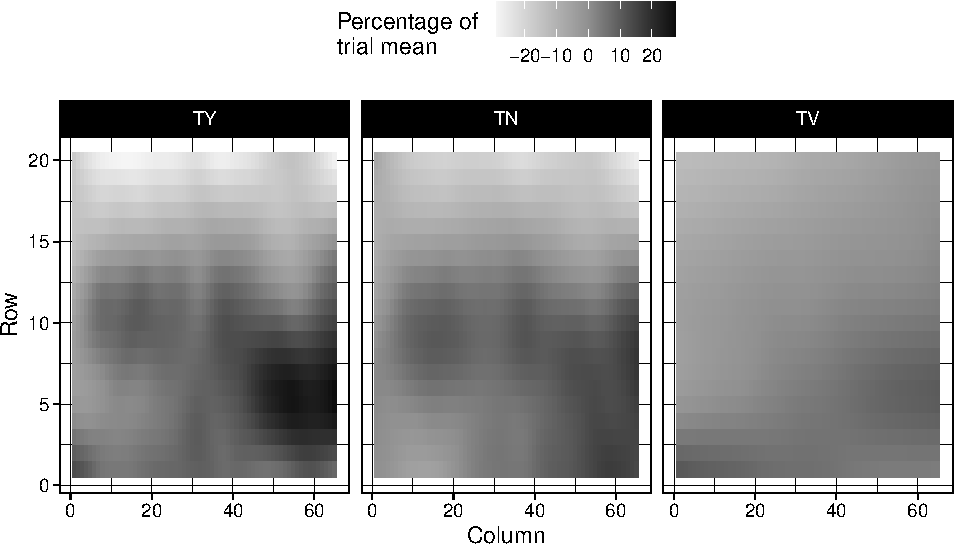
\includegraphics[width=\linewidth]{./figs_02/Fig1.pdf}
\caption{\label{fig:trend-est}Estimated spatial trends scaled by trial mean for total yield (TY; \(\frac{Mg}{Ha}\)) , tuber number (TN; Number of tubers per plot), and tuber volume (TV; Average \(cm^3\) per plot) within the Est screening trial.}
\end{figure}


\section{Results}

\subsection{Spatial Components}\label{spatial-components}

Spatial models for the Est and Heelsum trials were estimated for each yield component. All spatial models successfully converged with credible spatial trends for both trial locations. Model residuals for all environmental models showed little to no evidence of deviation from normality; the following suggest successful delineation of spatial components for all traits in both field trials.

Total yield and tuber number exhibited evidence for strong local trends with a row effect contributing to the spatial trend in Est (Figure \ref{fig:trend-est}). While these same components also impacted tuber volume, it was not nearly so prominent (See S1). The similar magnitude of row effects on tuber number and total yield can also be observed through the ratio of effective and nominal dimensions which were identical for these two traits (0.68) in contrast to tuber volume (0.47). Additionally, the effective nominal dimension ratio for hybrids (i.e.~a generalised heritability) was highest in tuber volume followed by total yield and lastly tuber number (See Table S1).

Overall, the spatial trends in the Heelsum trial were less severe than those evaluated in the screening trial in Est. Interquartile ranges of field effects were between -8.96\% and 9.04\% of the trial mean for total yield in Est while the range was -2.85\% and 3.55\% of the trial mean for yield in Heelsum (Figure \ref{fig:trend-hee}). The differences in magnitude of spatial components between these two trials were also similar for tuber number and tuber volume. Nonetheless, the estimated spatial components did have a modest effect on all yield related components in Heelsum. In particular, random effects for the field column had a minor impact on tuber volume (0.55), tuber number (0.48), and total yield (0.45) (See Table S2). General heritability estimates for Heelsum were akin to those observed in Est with values of 0.9, 0.82, and 0.88 for tuber volume, tuber number, and total yield, respectively.

\begin{figure}
\centering
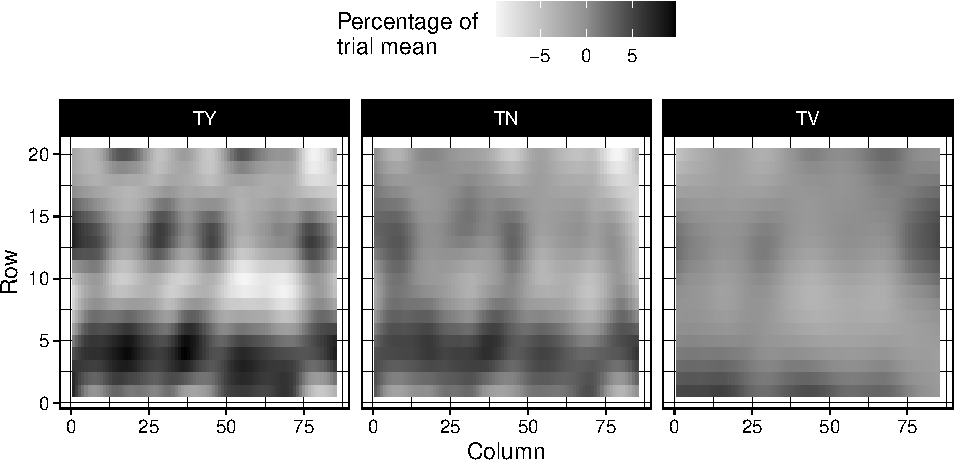
\includegraphics[width=\linewidth]{./figs_02/Fig2.pdf}
\caption{\label{fig:trend-hee}Estimated spatial trends scaled by their trial mean for total yield (TY; \(\frac{Mg}{Ha}\)) , tuber number (TN; Number of tubers per plot), and tuber volume (TV; Average \(cm^3\) per plot) within the Heelsum screening trial.}
\end{figure}

\subsection{Hybrid estimates}\label{hybrid-estimates}

    Using spatially corrected phenotypes from model \eqref{eq:general-spline-model}, we extracted both marginal and conditioned hybrid BLUP's from model \eqref{eq:hybrid} (Figure \ref{fig:blups-plot}). Generally, hybrid performance was far greater in Heelsum over Est. The trial mean for total yield was 13.1 and 22.4 \(Mg \cdot Ha^{-1}\) for Est and Heelsum, respectively. Likewise, average tuber number was 136 tubers in Est and 199 tubers in Heelsum. Trial means for tuber volume were comparatively more stable between trial locations with means of \(21.3~cm^3\) in Est and \(24.2~cm^3\) in Heelsum. Along with differences in mean hybrid performance, there was also greater dispersion of phenotypes in Heelsum than in Est. This was especially apparent for total yield in Heelsum which displayed a standard error twice the size of total yield in Est. This same marked difference could also be seen in tuber number where BLUP's in Heelsum exhibited a standard error 1.6 times greater than that which was found in Est. Tuber volume in contrast to the other phenotypes exhibited similar BLUP distributions between both trial locations. Examining these BLUP's in light of each trait's variance components (See Table S3) suggests that tuber volume showed the greatest stability of all three phenotypes.

    \begin{figure}
    \centering
    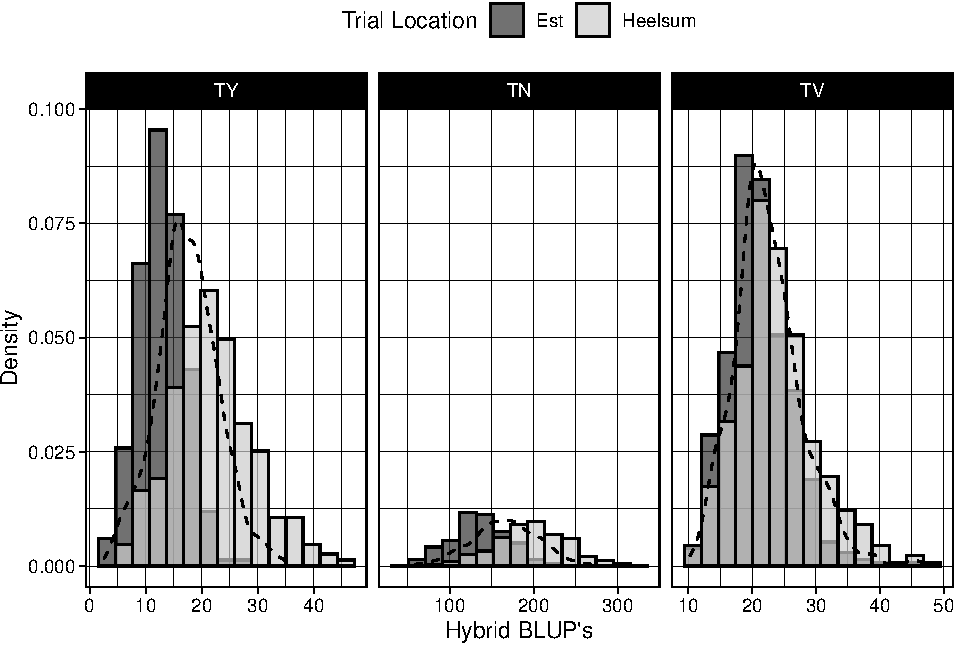
\includegraphics[width=\linewidth]{./figs_02/Fig3.pdf}
    \caption{\label{fig:blups-plot}Hybrid best linear unbiased predictions for total yield (TY; \(\frac{Mg}{Ha}\)) , tuber number (TN; Number of tubers per plot), and tuber volume (TV; Average \(cm^3\) per plot) conditioned on Est and Heelsum trials. Across-location BLUP's visualised through black density curve.}
    \end{figure}

\subsection{Variance Ratios}\label{variance-ratios}

        Variance estimates were derived for all specified random effects for models \(M_0\) and \(M_f\). Tuber volume not only exhibited the largest proportion of variance explained by SCA (\(d^2 = 0.14\)), but also had the largest total genetic variance of any trait (\(H^2 = 0.86\)) (Figure \ref{tab:ratio-tab}). Tuber number and total yield harboured similar proportion's of SCA (\(d^2 = 0.12\)) with a considerable portion of non-additive effects being partitioned in the SCA by environment interaction (Figure \ref{fig:plot-var}). Broad-sense heritabilities were quite similar between tuber number (0.74) and total yield (0.71) with the primary difference between the two traits being the partitioning of genotype by environment interactions (\(\frac{\sigma^2_{ae}}{\sigma^2_{GE}}\) equal to 0.78 in total yield in contrast to 0.65 in tuber number) and size of the residual variance (Figure \ref{fig:plot-var}). The additive genetic component was the largest genetic effect across all traits with the ratio of additive genetic variance being identitical in total yield and tuber number (0.84) and nearly identical in tuber volume (0.83). Between models \(M_0\) and \(M_f\), partitioning of variance changes most drastically for \(\sigma^2_{ae}\). These were much larger in \(M_f\) in tuber number and total yield with the incorporation of the SCA main effect and SCA by environment interaction (Figure \ref{fig:plot-var}).

        \begin{figure}
        \centering
        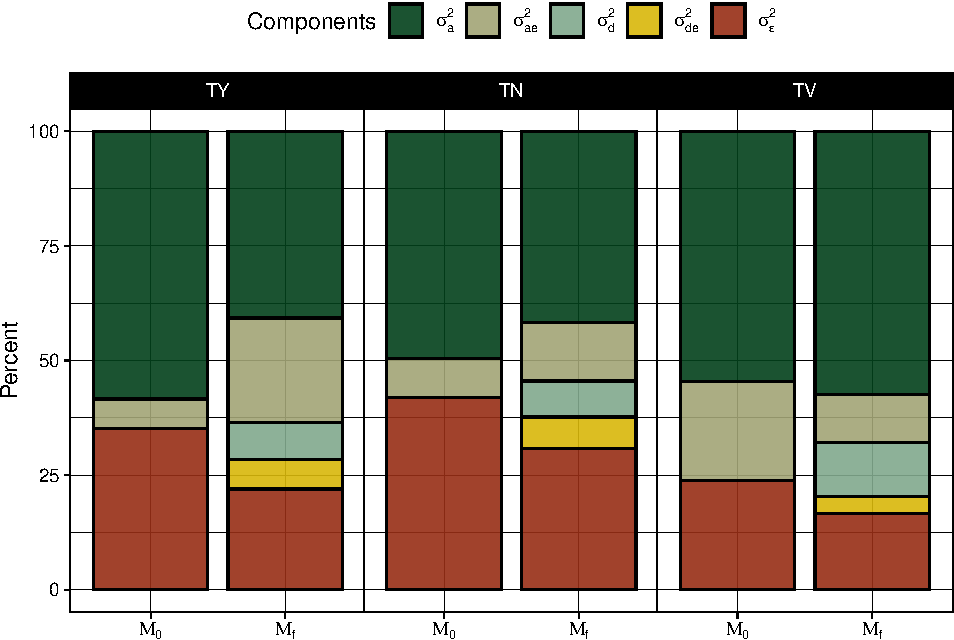
\includegraphics[width=\linewidth]{./figs_02/Fig4.pdf}
        \caption{\label{fig:plot-var}Partitioning of total phenotypic variance into additive (\(\sigma^2_a\)), dominant (\(\sigma^2_d\)), interactive (\(\sigma^2_{ae}\) \& \(\sigma^2_{de}\)), and residual (\(\sigma^2_\varepsilon\)) genetic components across each genetic model (\(M_0\) and \(M_f\)) for total yield (TY), tuber number (TN), and average tuber volume (TV).}
        \end{figure}

        \begin{table}

        \caption{\label{tab:ratio-tab}The broad and narrow-sense heritabilities ($H^2$ and $h^2$, respectively), dominance ratio ($d^2$), proportion of additive genetic variation ($\frac{\sigma^2_a}{\sigma^2_G}$), and proportion of additive genotype by environment interaction over total genotype by environment interaction ($\frac{\sigma^2_{ae}}{\sigma^2_{GE}}$) estimated from the $M_f$ model for total yield (TY), tuber number (TN), and average tuber volume (TV).}
\centering
\begin{tabular}[t]{cccc}
\toprule
 & TY & TN & TV\\
\midrule
$H^2$ & 0.71 & 0.74 & 0.86\\
$h^2$ & 0.59 & 0.62 & 0.71\\
$d^2$ & 0.12 & 0.12 & 0.14\\
$\frac{\sigma^2_{a}}{\sigma^2_G}$ & 0.84 & 0.84 & 0.83\\
$\frac{\sigma^2_{ae}}{\sigma^2_{GE}}$ & 0.78 & 0.65 & 0.74\\
\bottomrule
\end{tabular}
\end{table}

\subsection{Genetic correlations}\label{genetic-correlations}

Along with within-trait variance ratios, genetic correlations were also computed using covariances extracted from model \(M_f\). These were produced for GCA (Figure \ref{fig:gca-coef-full-pairs}) and SCA (Figure \ref{fig:sca-coef-full-pairs}) and are shown together with their BLUP distribution for reference. The GCA intra-class correlation coefficient was found to be highest in tuber volume (0.84) followed by tuber number (0.76) and total yield (0.64) (Figure \ref{fig:gca-coef-full-pairs}). Also noteworthy, large within-trial GCA genetic correlations were found between total yield and each of its yield components, tuber number (0.80) and tuber volume (0.64) according to expectation. Little to no genetic correlation could be found between tuber number and tuber volume (0.06). There were minor discrepancies when comparing each of these with their between-trial genetic correlations counterparts (\(\rho_{TY,TN} = 0.81, \rho_{TY,TV} = 0.65, \rho_{TN,TV}=0.11\)).

\begin{figure}
\centering
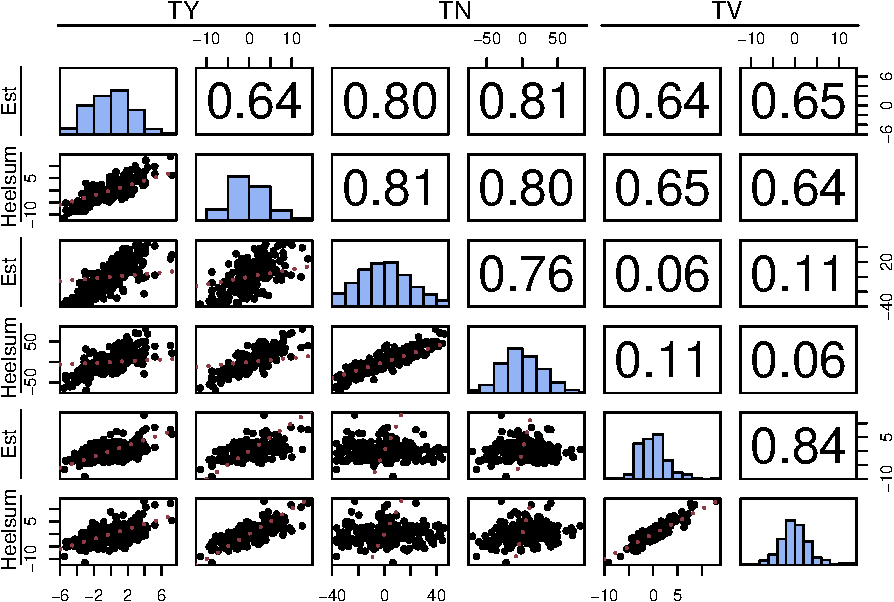
\includegraphics[width=\linewidth]{./figs_02/Fig5.pdf}
\caption{\label{fig:gca-coef-full-pairs}General combining ability pairwise comparisons with scatterplot (lower triangle), genetic correlations derived from \(M_f\)'s variance components (upper triangle), and marginal distributions (the diagonal) of best linear unbiased predictions for total yield (TY; \(\frac{Mg}{Ha}\)), tuber number (TN; total number of tubers per plot), and average tuber volume (TV; \(cm^3\)) in Est and Heelsum. The identity is provided in red for each scatterplot (lower triangle).}
\end{figure}

Similar multivariate trends were observed for SCA genetic correlations, though, with globally smaller values. The SCA intra-class correlation was highest in tuber volume (0.75) with little difference between total yield (0.55) and tuber number (0.53) (Figure \ref{fig:sca-coef-full-pairs}). Relatively large within-trial genetic correlations were observed between total yield and tuber number (\(\rho_{TY,TN} = 0.73\)) and between total yield and tuber volume (\(\rho_{TY,TV} = 0.69\)). Genetic correlations between tuber number and tuber volume were virtually null (\(\rho_{TN,TV}=0.03\)) showing little to no covariance between these two traits for SCA. Examining between-trait between-trial correlations only had minor deviations with respect to within-trial genetic correlations between total yield and tuber number (\(\rho_{TY,TN}=0.76\)) and tuber number and tuber volume (\(\rho_{TN,TV}=-0.01\)); however, these correlations between total yield and tuber volume were distinctly smaller than their within-trial counter-parts (\(\rho_{TY,TV}=0.55\)) (Figure \ref{fig:sca-coef-full-pairs}).

\begin{figure}
\centering
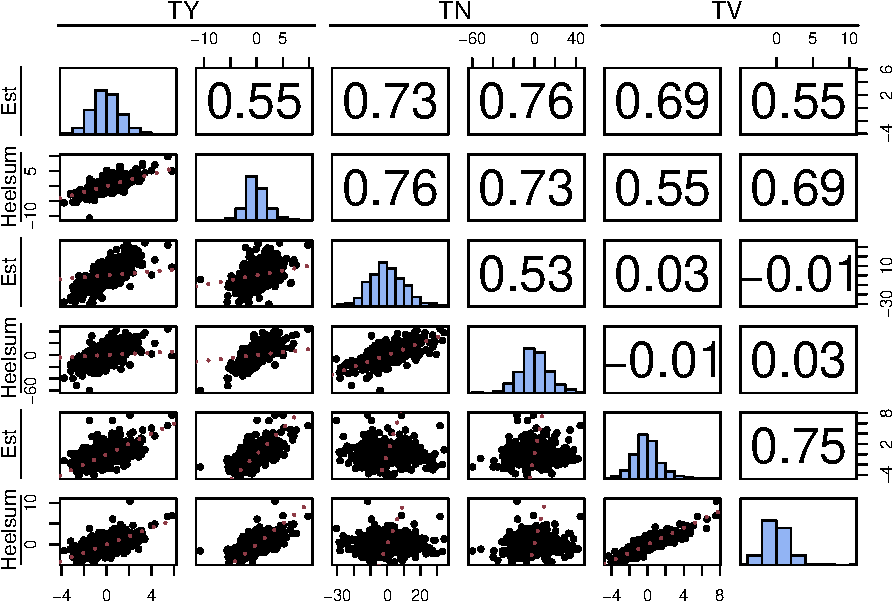
\includegraphics[width=\linewidth]{./figs_02/Fig6.pdf}
\caption{\label{fig:sca-coef-full-pairs}Specific combining ability pairwise comparisons with scatterplot (lower triangle), genetic correlations derived from \(M_f\)'s variance components (upper triangle), and marginal distributions (the diagonal) of best linear unbiased predictions for total yield (TY; \(\frac{Mg}{Ha}\)), tuber number (TN; total number of tubers per plot), and average tuber volume (TV; \(cm^3\)) specific combining ability in Est and Heelsum. The identity is provided in red for each scatterplot (lower triangle).}
\end{figure}

When comparing the GCA and SCA quantiles for each trait and trial location, the GCA BLUP's were consistently larger than those SCA BLUP's. On average, any given GCA quantile was two times larger than its respective SCA quantile; this was true for all traits measured here (See Table S4). These differences in magnitude between the estimated GCA and SCA effects could also be readily seen while examining the size of each variance component (Figure \ref{fig:plot-var}) or even through a simple regression of hybrid BLUP's on the mid-parent value (Figure \ref{fig:bv-sca}). No linear relationship could be found between the estimated GCA and SCA effects for any trait (See Figure S1) coinciding with our model assumptions in   \eqref{eq:sca-model}.

\begin{figure}
\centering
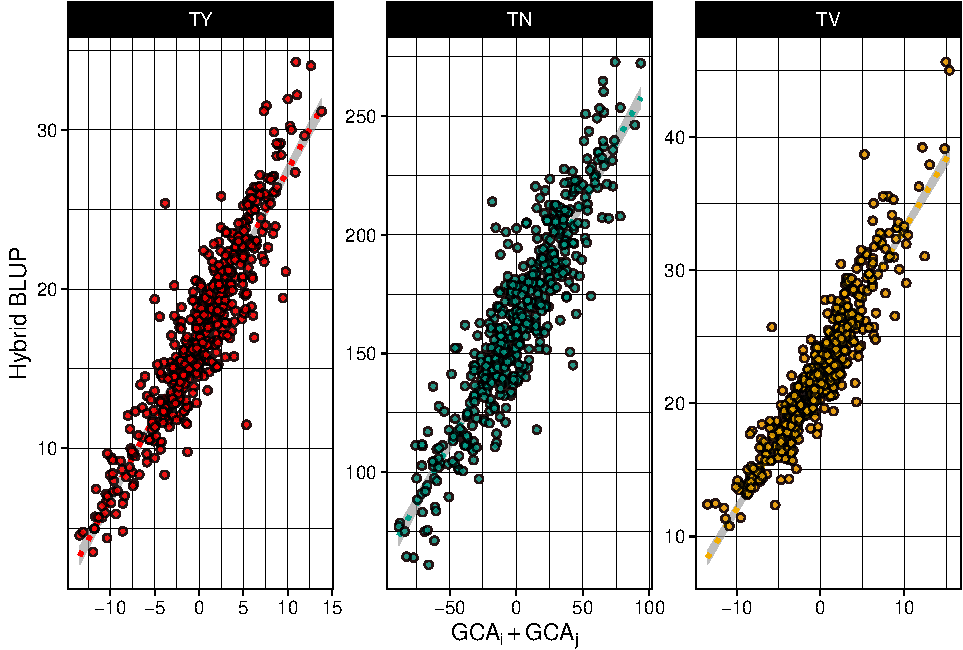
\includegraphics[width=\linewidth]{./figs_02/Fig7.pdf}
\caption{Scatterplot of hybrid BLUP's regressed on the GCA's of parents' i and j for total yield (TY; \(\frac{Mg}{Ha}\)), tuber number (TN; total number of tubers per plot), and average tuber volume (TV; \(cm^3\))}
\label{fig:bv-sca}
\end{figure}

\subsection{Model Testing}\label{model-testing}

The likelihood ratio tests conducted between model \(M_f\) and \(M_0\) was found to be significant yielding a probability less than 0.001 (Table \ref{tab:model-comparison}). This test was also conducted on the univariate equivalent of these models for each trait (\(M_{df}\) and \(M_{d0}\)) and were all found to be significant as well. Each test conformed with the AIC's of each model pair where the smallest AIC was observed in the full genetic model suggesting that the best fit was achieved with the inclusion of SCA and its environmental interaction. This at the very least lend a statistical justification for these non-additive genetic effects in all three tuber traits.

\begin{table}

\caption{\label{tab:model-comparison}Likelihood ratio tests for $M_0$ and $M_f$ genetic models together with each model's Akaike's information criterion for the Multi-trait model (MT), total yield (TY), tuber number (TN), and average tuber volume (TV).}
\centering
\begin{threeparttable}
\begin{tabular}[t]{cccc}
\toprule
 & AIC & $\Lambda(y)$ & $\mathrm{P}(\Lambda(y))$\textsuperscript{\dag}\\
\midrule
\addlinespace[0.3em]
\hline
\multicolumn{4}{l}{\textbf{MT}}\\
\hspace{1em}$M_0$ & 26665 & 586 & ***\\
\hspace{1em}$M_f$ & 26103 &  & \\
\addlinespace[0.3em]
\hline
\multicolumn{4}{l}{\textbf{TY}}\\
\hspace{1em}$M_0$ & 7992 & 132 & ***\\
\hspace{1em}$M_f$ & 7864 &  & \\
\addlinespace[0.3em]
\hline
\multicolumn{4}{l}{\textbf{TN}}\\
\hspace{1em}$M_0$ & 15778 & 92 & ***\\
\hspace{1em}$M_f$ & 15690 &  & \\
\addlinespace[0.3em]
\hline
\multicolumn{4}{l}{\textbf{TV}}\\
\hspace{1em}$M_0$ & 7008 & 235 & ***\\
\hspace{1em}$M_f$ & 6778 &  & \\
\bottomrule
\end{tabular}
\begin{tablenotes}
\item[\dag] ***: $\mathrm{P}(\Lambda(y))< 0.001$
\end{tablenotes}
\end{threeparttable}
\end{table}

\section{Discussion}\label{discussion}

\subsection{Presence of additive vs.~non-additive effects}\label{presence-of-additive-vs.-non-additive-effects}

SCA was detected across all phenotypes (Table \ref{tab:model-comparison}) warranting sufficient evidence that SCA can impact yield, especially in its simpler components, seen primarily in tuber volume (Figure \ref{fig:plot-var}). However, the magnitude of GCA effects were far greater than the magnitude of SCA's estimated across all traits irrespective of the their heritability or size of SCA variance. The GCA quantiles were between 1.4 to 2.5 times larger than their respective SCA quantiles (See Table S4) suggesting a systematic importance of the additive genetic effects in this DHP population. The implications then is that most of the variation in the progeny can be found through the additive genetic variation in the parents. This was most apparent for tuber volume (\(h^2 = 0.71\)) where regression of hybrid performance on the combination of parental GCA's had the best fit of all traits (Figure \ref{fig:bv-sca}). This illustrates that the parental GCA's (or, identically, the mid-parent value) capture the majority of a hybrid's phenotype.

While this study is the largest of its kind, it is certainly not alone in attempting to decompose genetic components of yield in potato. A number of similar populations were used in both diploid and tetraploid backgrounds with wide-ranging results. Many of these studies came to find little non-additive genetic variation for yield components similar to the results presented here with GCA being the primary component for traits like average tuber weight, tuber shape, total tuber number, and total yield \citep{Veilleux1981, Brown1989, Neele1991}. These studies utilised either variants of a diallel or factorial crossing schema making the structure of their statistical models not altogether different than the modelling endeavoured here. One exception between models' \eqref{eq:gca-model} and \eqref{eq:sca-model} and those used in the aforementioned tetraploid populations is that variance attributed to GCA has a different interpretation due to differences in ploidy and levels of inbreeding. This said, there is a large body of work which also finds SCA to be the largest (and at times, the only) detected effect in several complex traits. The same previously mentioned traits as well as others like incidence of hollow heart and tuber uniformity were also found to be predominately under the control of SCA \citep{Killick1977, Veilleux1981, Thompson1984, Haynes2001}. Most notably, \citep{Tai1976} was only able to detect SCA in their partial diallel crosses with no GCA component found for marketable yield and marketable tuber number.

The lack of an empirical consensus on the predominance of GCA and SCA in potato is not very surprising in of itself. The estimation of these parameters are very much contingent on numerous factors including crop ploidy, genetic background, number of parents, degree of environmental stress, and choice of statistical model (to name a few), all of which are prone to change across experiments. Even making comparisons between studies utilising very similar genetic backgrounds can lead to divergent findings \citep{Tarn1977, Maris1989}. While seemingly incoherent, the following does offer some interesting grounds for considering those genetic effects observed here. Many of the aforementioned studies estimated variance components on populations which had undergone siginificant selection through a recurrent selection schema \citep{Haynes2001, Maris1989} or were themselves the product of strong selection on GCA's in their ancestors \citep{Tai1976}. In both cases, less additive genetic variation can be expected among hybrids derived from them leaving non-additive genetic variation to be the predominant genetic effect within their inter-population crosses. Conversely, populations like ours which show ample additive genetic variation might be younger with respect to selection pressure in their ancestors on these traits; though without any formal analysis on population structure this is speculative. Another line of reasoning for the smaller SCA's found here relative to many of the tetraploid studies could be explained by \emph{progressive heterosis} whereby higher order non-additive genetic effects become possible through polyploidy \citep{Birchler2003}. Recent genomic studies in tetraploid potato support this hypothesis with evidence of a genetic residual effect (which could be explained by tri \& quadrigenic dominance) contributing as much as 45\% of total genetic variation in potato yield \citep{Endelman2018}. However, making any meaningful confirmation on the specific role of ploidy in producing non-additive genetic effects is beyond the scope of this present study and only deserves a cursory mention.

\subsection{Genetic Architecture of yield}\label{genetic-architecture-of-yield}

Among our two yield components (i.e. tuber number and and average tuber volume), we found strong genetic correlations between each and total yield for both the additive (see Figure \ref{fig:gca-coef-full-pairs}) and non-additive genetic effects (see Figure \ref{fig:sca-coef-full-pairs}). Numerous studies have identified these same phenotypes as major determinants of total tuber yield marking them both as strategic heritable targets for breeding \citep{Khayatnezhad2011, Thompson1984}. Consistent with these studies, tuber number GCA's appeared to impact total yield more than tuber volume with \(\rho_{TN,TY}\) equalling 0.80 and a \(\rho_{TV,TY}\) of 0.64. SCA genetic correlations behaved similarly with \(\rho_{TN,TY}\) equal to 0.73 and \(\rho_{TV,TY}\) equal to 0.69. Interestingly, while tuber volume had the greatest stability with respect to both GCA (\(ICC_{gca}=0.84\)) and SCA (\(ICC_{sca}=0.75\)), the between-trial genetic correlations in \(\rho_{TV,TY}\) dropped to 0.55 suggesting less coupling in SCA by trial response with total yield in contrast to the between-trial genetic correlations seen in total yield and tuber number (\(\rho_{TN,TY}\)=0.76). These additive and non-additive components point to tuber number being the primary determinant of yield in this hybrid population.

Among certain market classes, our two yield components, average tuber volume (or tuber size) and tuber number, often exhibit an inverted relationship due to the physiological and genetic limits of potato. For example, \citep{Thompson1984} found a genetic correlation of -0.24 among their panel. Additionally, \citep{Lemaga1990} identified negative cubic trends between tuber number and average tuber weight capturing a majority of variation. Interestingly, no meaningful relationship could be found between these two yield components with respect to additive (Figure \ref{fig:gca-coef-full-pairs}) and non-additive genetic correlations (Figure \ref{fig:sca-coef-full-pairs}). To repeat our previous suspicion, this suggests a lack of directional selection on one of these two traits evident by the lack of genetic constraints between them \citep{Blows2009}. Tuber volume had the largest proportion of additive variation (Figure \ref{fig:plot-var}) and genetic variation in general (Table \ref{tab:ratio-tab}) suggesting little to no direct selection on this component of yield. These properties then make this population an interesting candidate for future selection given its genetic potential to be adapted to a variety of tuber types. Another oddity to consider here is that while SCA was detected independently in these two yield components, this did not manifest in the increase of SCA in total yield, but very much the opposite. Others have identified that heterosis in these same yield components were responsible for a geometric increase in gross yield \citep{Tarn1977}. Further multivariate studies of vigour in diploid potato could further elucidate SCA architecture especially as selection pressure is applied, a key scenario within breeding programmes.

\subsection{Using GCA \& SCA in commercial breeding}\label{using-gca-sca-in-commercial-breeding}

The large narrow-sense heritabilities and magnitude of the GCA's found here have major implications for breeders of DHP. To begin, the valid estimation of GCA's further validate the potential of potato in its conversion into a inbred-hybrid crop as purported before \citep{Jansky2016, Lindhout2011}. Further, the size of the estimated GCA's relative to a hybrid's average performance (Figure \ref{fig:bv-sca}) show that standard breeding designs used in other hybrid crops will likely be just as efficacious in DHP. For example, the use of test crosses, a mainstay in maize breeding, can also be utilised in evaluating performance of potato parental lines for hybrid crosses with reasonable success. These test crosses can be further utilised for model training and be the basis for genomic selection of parents (using breeding values) or hybrid crosses (via mid-parent value); again, a standard-place method in hybrid breeding \citep{Albrecht2011}. To quickly add, while we found little contributions made by SCA, their relevance to breeders do not necessarily end here. Depending on the specific mechanism behind these observed non-additive effects, they could be further exploited in the trait of interest through initial breeding design (e.g.~formation of heterotic pools). Heterotic breeding has become a major target for quality trait improvement in other solanaceous crops including chilli pepper \citep{Herath2020}, eggplant \citep{Kumar2020}, and tomato \citep{Pearson1983}. This is where potato meets an interesting intersection between the vegetable and agronomic worlds where SCA might play a more valuable role for qualities controlling specific market criteria (e.g.~average tuber volume, tuber length \& shape) but would be less emphasised in composite and complex traits (e.g.~gross yield, starch \& protein content) where GCA is the predominant genetic effect at play. Having said this, future work into the biometric mechanism of vigour will be able to lend more wisdom for how breeders should wield this in a hybrid potato breeding programme.



\section{Conclusion}\label{conclusion}

\subsection{Limitations}\label{limitations}

The application of these results should be done with some qualification. One principal limitation of this study can be found in the number of trials conducted. All inference drawn here was based upon only two trials which took place over one season. This limits our findings to one particular year which narrows their interpretive weight and scope. Related to this, this study was performed on a particular composite experimental population and does not necessarily represent the heterotic potential of the tuber-bearing Solanum genepool. Considering all this, this population is an appropriate candidate for the purpose of surveying the presence and potential of heterotic vigour in DHP which was the aim of this current paper. 

\subsection{Future work}\label{future-work}

Finding evidence for heterotic effects in DHP does not yield much regarding the source of the effects identified here. The statistical models assume all underlying effects captured by the SCA term to be the product of cumulative dominance deviations across the genome, but there exists many other plausible sources of non-additive variation. Since its conception, genetic theory has explained heterosis with a whole suite of models with many being broadly plausible (See \citep{Labroo2021}). However, these apparent non-additive effects could just as simply be explained by dispersion of additive alleles among parents, a hypothesis which is generally supported empirically \citep{Pearson1983, Mackay2021}. Nevertheless, these effects continue to be interesting point of study and still remain an important target in hybrid breeding of modern crops. This is especially worthwhile in DHP given its novelty as a hybrid crop with the potential of heterotic breeding to still be determined.


This is the first study in diploid hybrid potato to produce estimates of general and specific combining abilities using a large panel of commercially-derived parents. This represents a major milestone in the reorientation of potato from a clonal tetraploid to a diploid inbred-hybrid crop. Identifying the predominance of additive genetic effects for multiple yield components among hybrids offers strategic insight on the necessity of effective generation of parental lines and early population development in general. Though the estimated non-additive effects in this population are smaller in contrast to their additive counterparts, heterotic vigour shows some minor role in simpler traits. Specific quantitative traits should be targeted for SCA exploitation to bolster variety development on top of their parental effects. Further research into the genetic mechanisms for the apparent non-additive effects will also better elucidate the strategic advantage (if any exist) in key economic targets in hybrid potato.

\section{Data availability}

All trial and pedigree data utilised for the following analysis have been made
available on GSA FigShare. File Phenotypes.csv contains the three afore-
mentioned traits along with field trial row, column, and block indices for each
observation. File Pedigrees.csv gives a hybrid identification number with
each parental code.

\section{Acknowledgments}
Acknowledgments should be included here.

\section{Funding}
Funding, including Funder Names and Grant numbers should be included here.

\section{Conflicts of interest}

The authors of this publication have no conflicts of interest to report related to the the results of this study or the inferences, speculation,\& conclusions derived from them.


\chapter[Efficient genomic prediction of yield and dry matter in hybrid potato]{Efficient genomic prediction of yield and dry matter in hybrid potato}

\chaptermark{Efficient genomic prediction of yield and dry matter in hybrid potato}
\label{cha:chapter3}
\vspace*{\fill}
This chapter is based on:
\\
\\
% Full citation of the published (or submitted/in review) article
% This refers to the article key in the refs.bib file.
\bibentry{Adams2023}
\newpage

\section*{Abstract}

There is an ongoing endeavor within the potato breeding sector to rapidly adapt potato from a clonal polyploid crop to a diploid hybrid potato crop.  While hybrid breeding allows for efficient generation and selection of parental lines, it also increases breeding program complexity and results in longer breeding cycles. Over the past two decades, genomic prediction has revolutionized hybrid crop breeding through shorter breeding cycles, lower phenotyping costs, and better population improvement resulting in increased genetic gains for genetically complex traits. In order to accelerate genetic gains in hybrid potato, proper implementation of genomic prediction is a crucial milestone in the rapid improvement for this crop. The authors of this paper set out to test genomic prediction in hybrid potato using current genotyped material with two alternative models: one model that predicts the general combining ability effects (GCA) and another which predicts both general and specific combining ability effects (GCA+SCA). Using a training set comprised of 769 hybrids and 456 genotyped parental lines, we found that reasonable prediction accuracy's could be achieved for most phenotypes with both zero common parents (\(\rho = 0.36 - 0.61\)) and one ($\rho = 0.50 - 0.68$) common parent between training and test sets. There was no benefit with the inclusion of non-additive genetic effects in the GCA+SCA model despite SCA variance contributing between 9\% and 19\% of total genetic variance. Genotype by environment interaction, while present, did not appear to affect prediction accuracy's though prediction errors did vary across trial targets. These results suggest that genomically estimated breeding values on parental lines are sufficient for hybrid yield prediction.


\newpage

% Keywords
\keyword{Hybrid potato; genomic prediction; general combining ability; genomically estimated breeding values; Hybrid prediction; genomic prediction; Genotype by environment} 

\section{Introduction}

Potato (\textit{Solanum tuberosum} L.) is the most important starch source among vegetable crops. Cultivated for its edible tubers, potato's end-use spans across multiple markets including table, chipping, frying, and industrial processing with a global export value of 3.36 billion USD \cite{fao2023}. It has positive production characteristics including excellent water use efficiency and short crop cycles making it amenable to a variety of cropping systems \cite{Haverkort1990}. Despite potato's potential for food systems worldwide, slower genetic progress, particularly for quantitative traits such as yield, is a known impediment to long-term food security \cite{Douches1996}. Underlying factors are numerous, but this is understood to be the consequence, in part, by potato's polyploidy and large genetic load \cite{Lian2019}. In the context of breeding, this makes potato an obligate outcrosser and affects the whole breeding system from initial crosses to the selection schemas used in identifying favourable varietal candidates. Together with potato's large selection surface (as many as 40 traits), improving quantitative traits in clonal potato is rife with technical difficulties \cite{Gebhardt2013, Gopal2015}.  

There have been many proposed (and implemented) innovations for conventional clonal breeding including the use of marker-assisted selection, progeny testing strategies, and genetic transformation  \cite{Bradshaw2022}. Among these, one topic which has garnered significant interest over the past few decades is adapting tetraploid potato (2n = 4x = 48) to a diploid hybrid breeding system (2n = 2x = 24) \cite{Lindhout2011, Jansky2016}. The appeal of diploid hybrid potato (DHP) breeding is understood to consist of benefits such as the use of true potato seed (TPS) directly in varietal evaluation \cite{VanDijk2021}, segmented breeding program design \cite{Technow2021}, exploitation of heterotic vigour \cite{Technow2012}, and more efficient systems for germplasm production and dissemination \cite{Pallais1991}. With the gradual emergence of fertile diploid lines \cite{Eggers2021, Ma2021}, research centered around diploid and hybrid potato breeding are gaining momentum across the world \cite{Lindhout2018, Bethke2022, Jansky2016, Zhang2021}. 

With all of hybrid breeding's benefits, it is also known for being more resource and time intensive in contrast to inbred systems \cite{Labroo2021}. Hybrid breeding systems are also more complex in terms of breeding targets; not only must the breeder find the best set of parents (targeting general combining ability, i.e., GCA), but also find the best cross among that set of parents (targeting specific combining ability, i.e., SCA). Because of this, genomic prediction (GP) and genomic selection (GS) have become indispensable methods in the implementation of hybrid breeding in multiple crops \cite{Zhao2015a, Labroo2021}. The wide-spread adoption of these techniques have been made possible through the advent of high-throughput molecular marker data and the availability of powerful computational resources capable of rapid model fitting \cite{Meuwissen2001, Bernardo2016}. These methods are conceptual extensions of marker-assisted selection where rather than selecting an individual on its' QTL status, selection is on the basis of genome-wide estimated breeding values (GEBV's). GP and GS have been used to increase the efficiency of hybrid breeding through better heterotic pool development \cite{Rembe2019}, intra-population improvement \cite{Gaynor2017}, and even shortening breeding cycles by forgoing trialling altogether \cite{Heffner2010}. Because of GP and GS's demonstrated gains in hybrid, and crop breeding more generally, developing appropriate models for each target trait with adequate training sets is a major pursuit in any breeding endeavour. 

Recently, GP has received much attention in tetraploid potato with encouraging results demonstrated in chipping quality \cite{Sverrisdottir2018, Pandey2022}, disease resistance \cite{Enciso-Rodriguez2018, Ortiz2022},fry colour \cite{Byrne2020}, dry matter content and specific gravity \cite{Endelman2018, Sverrisdottir2018}, yield components \cite{Endelman2018, Wilson2021, Ortiz2022, Cuevas2022}, and vine maturity \cite{Slater2016, Pandey2022}. Despite the increased interest in breeding DHP, there are currently no analogous studies confirming model performance for economically valuable traits. Additionally, while targeting the general combining ability (GCA) gives acceptable prediction accuracy's in both simulation studies and \textit{in situ} for many crops, evaluating the contribution of non-additive effects (often through specific combining ability, i.e., SCA) is an altogether crucial question in GP's implementation. The authors of this study wish to showcase GP in DHP with three primary aims. First, to demonstrate the feasibility of GP for hybrid performance of multiple yield components and tuber dry matter content. The second, to test for the contribution of additive and non-additive genetic effects for each tuber phenotype. Lastly, a cursory examination on genotype by environment effects to understand their impact on prediction among the trials used in this study. Prediction models were constructed by adapting the modelling procedure of \cite{Adams2022} by structuring the random genetic effects with marker information. Through this work, we touch upon several facets of predictive breeding, all of which, are crucial for adoption and improvement of hybrid potato within the wider potato industry.


\section{Material and methods}

\subsection{Populations \& Trials}

Between 2017 and 2020, several crossing blocks were constructed around 712 experimental inbred lines sourced from Solynta, a Dutch hybrid potato breeder \cite{Lindhout2018}. These lines were generated from an original population comprised of 16 founders and selected primarily based on tuber criteria as well as on fertility characteristics during inbreeding. Across five nurseries, 1,162 hybrids were produced through a sparse mating design, i.e., only a small fraction of crosses were conducted over the full crossing space (\(n^2\)) \cite{Wang2020}. Hybrid TPS from these crosses were sown in trays in early-March and transplanted in mid-May in both trial years. These hybrids were transplanted in all four field trials in two trial locations (Heelsum and Est, Netherlands) in 2019 and 2020. The trials conducted in 2019 tested the performance of 806 F1 crosses, as previously described in \cite{Adams2022}, with 356 additional hybrids evaluated in 2020 with a thin intersect of hybrids between years (43 hybrids) and thinner intersect across all trials (25 hybrids). All trials utilised a double ridge design comprising of 16 plants per plot; ridges were 75 cm wide with plants spaced 25 cm within the same ridge. Each trial utilised a randomised complete block design consisting of two replicates for each hybrid with additional control varieties planted in diagonals across blocks for spatial trend control. Haulm killing took place in September with subsequent harvests occurring two weeks later. All tubers excluding those smaller than the 20 mm size class (due to instrumentation constraints) were harvested and measured on multiple traits including total tuber yield (TY; \(\mathrm Mg \cdot \mathrm{Ha^{-1}}\)), total tuber number (TN; \(\mathrm{number~of~tubers~per~plot)}\)), percentage of tuber dry matter content (DM; per cent), and average tuber volume (TV; \(cm^3\)). All phenotyping procedures, trait definitions, and instrumentation used here are described in \cite{Stockem2020}.

\subsection{Marker Processing and Analysis}

The parental lines used for test-crosses were genotyped using a targeted genotyping-by-sequencing (GBS) technology, SeqSNP\textsuperscript{®} \cite{LGC2019}. These probes were designed around highly conserved regions across the genome. Per LGC's protocol, leaf disks were sampled from each inbred line and placed in a 96-well plate and sent to LGC for DNA extraction and analysis. Upon reception of results, marker quality was assessed primarily on confirming coverage and read depth for each sample. For the purpose of this study, these probes were filtered for high-quality biallelic SNP's using multiple criteria. These included typical filtering criteria such as minor allele frequency (\(p \ge 0.05\)), percentage of SNP missingness (\(m \le 0.1\)) along with polymorphism information content (PIC) and linkage disequilibrium (LD) between sites. The latter was chosen due to high LD between many SNP's resulting in redundant marker information. A SNP selection procedure was invoked using the \(r^2_v\) metric provided by \cite{Mangin2012} which accounts for shared population history which tends to bias the traditional \(r^2\) statistic.  For any site in high LD with another (\(r^2_v \ge 0.5\)), the site with the highest PIC was chosen. This resulted in a filtered probe set containing 704 SNP's. There was a fraction of parental lines that were either genotyped with an irrelevant probe set or not genotyped at all. This resulted in 456 of the original 712 parental lines being present in the marker set.

\begin{figure}[H]
\begin{adjustwidth}{-\extralength}{0cm}
\centering
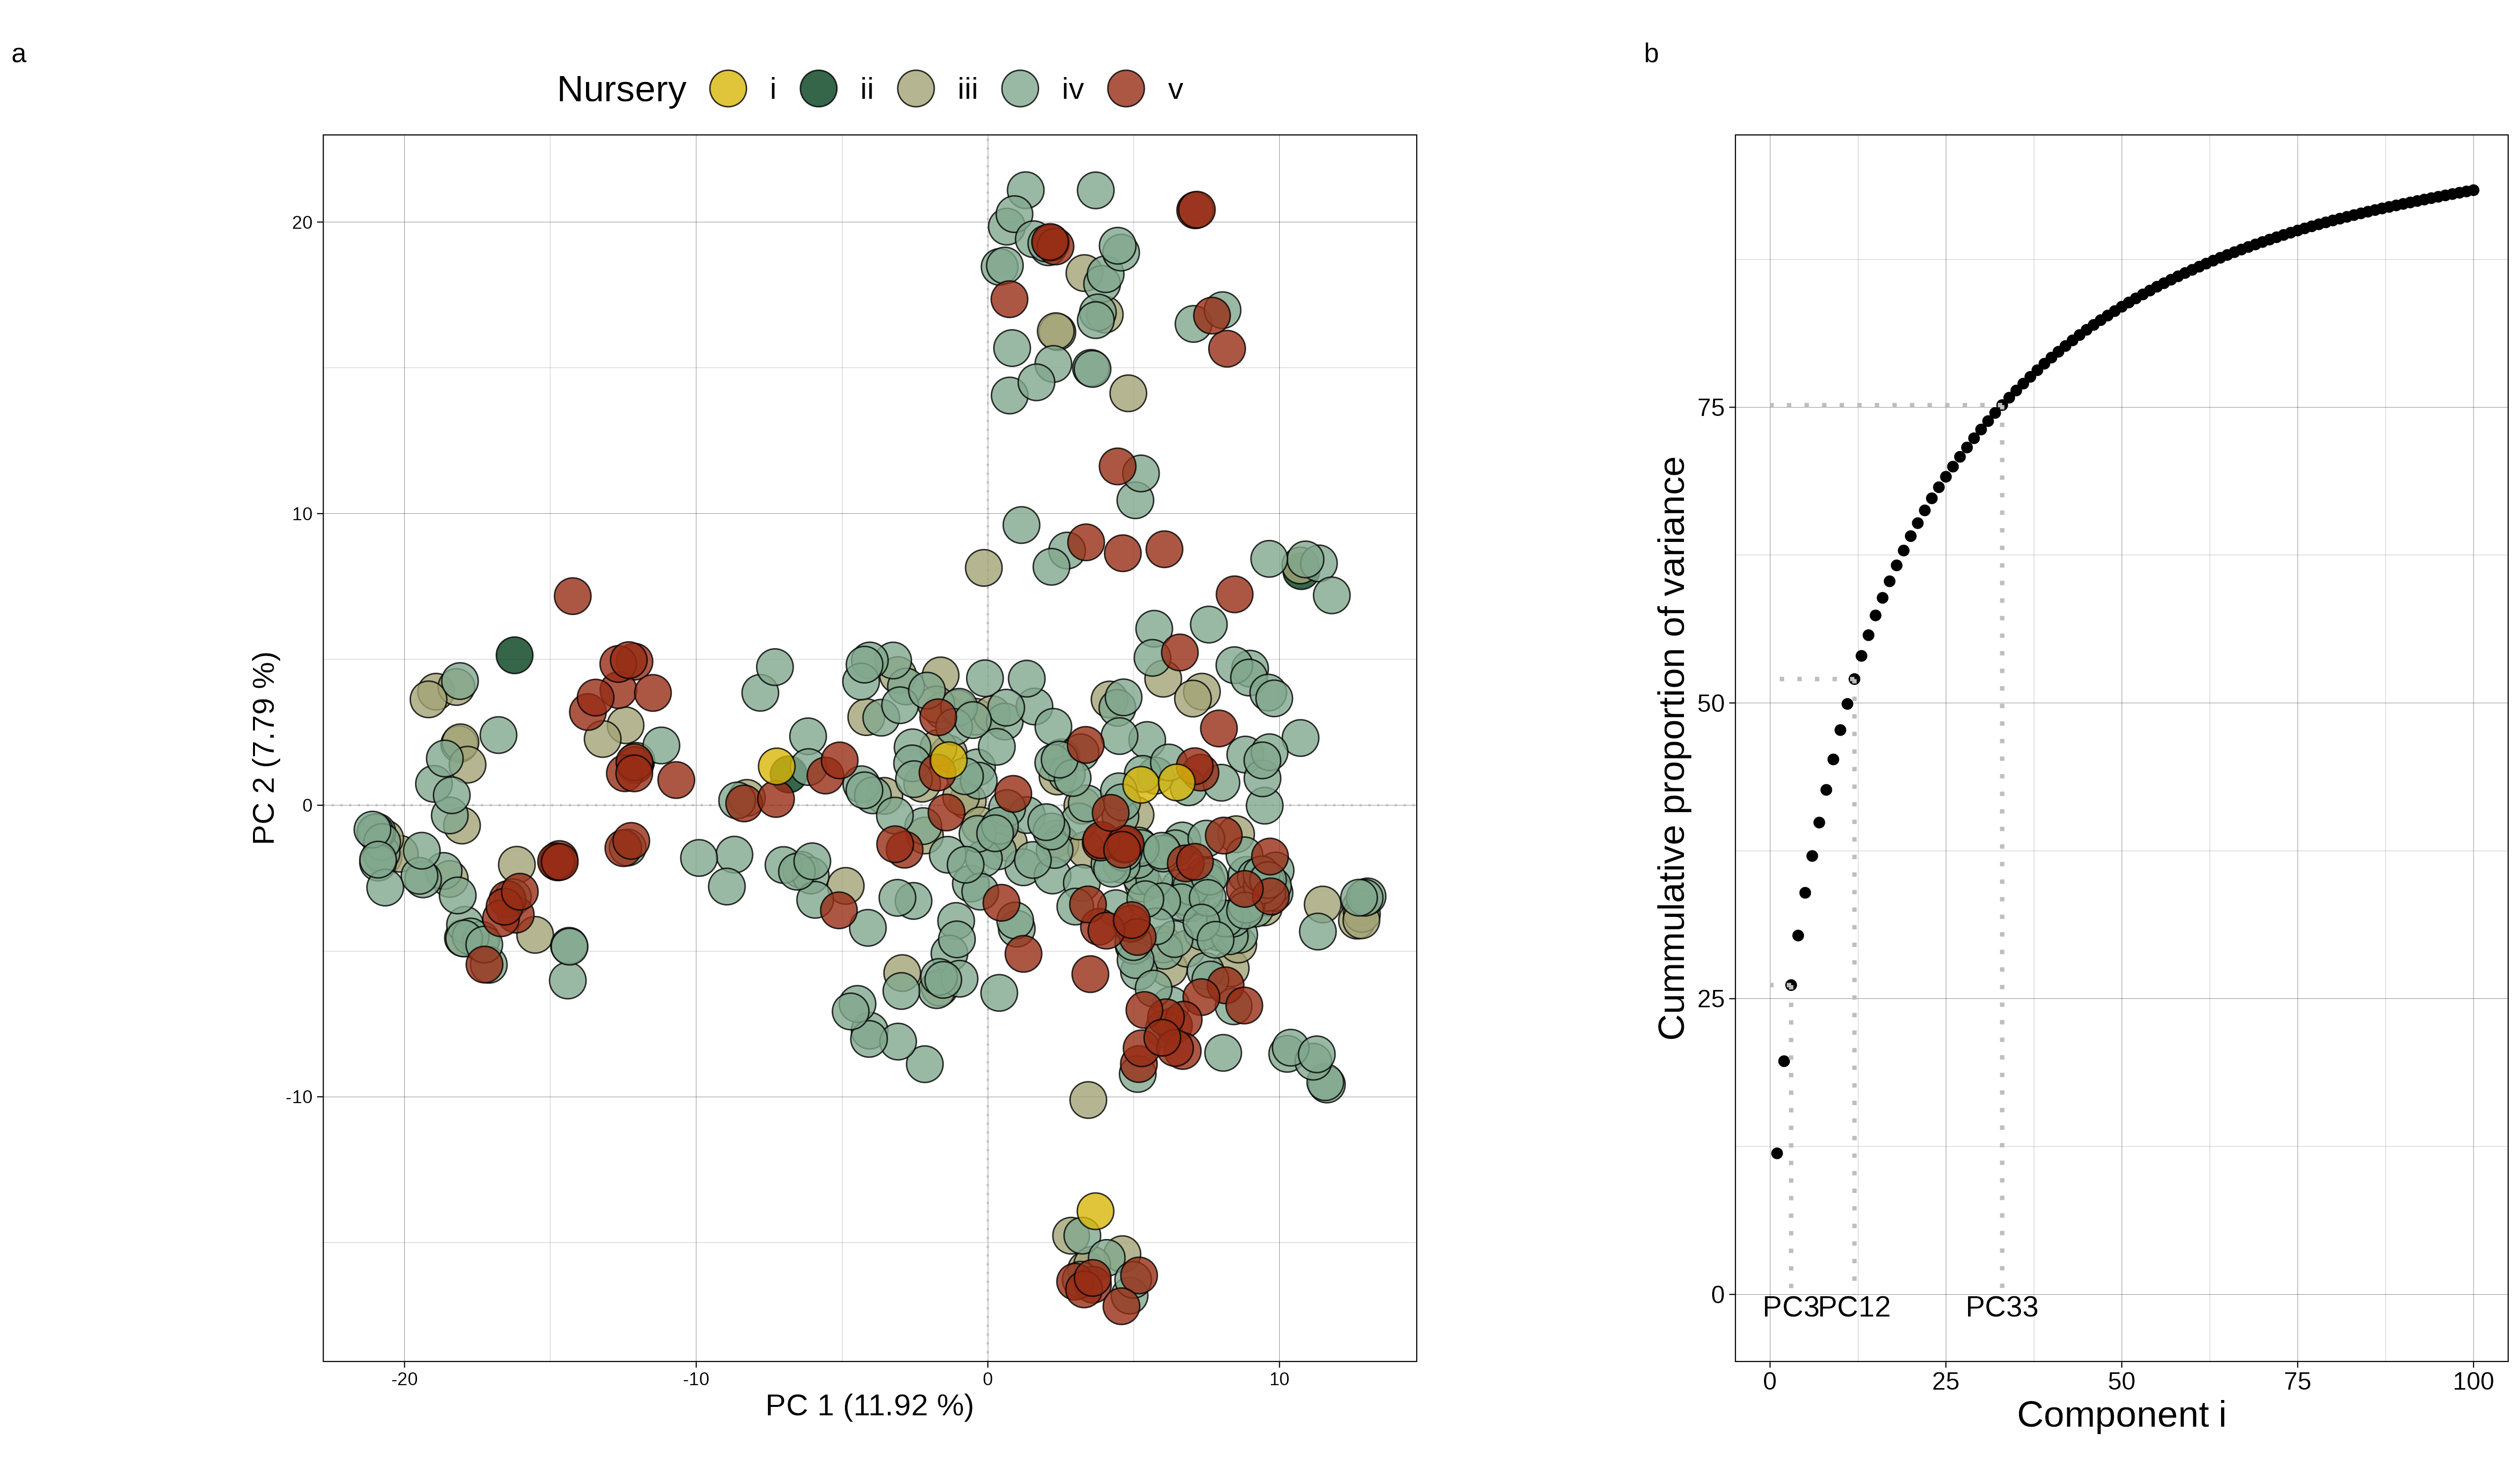
\includegraphics[width=15.5cm]{figs_03/1664970293popPca.png}
\end{adjustwidth}
\caption{(a) Principal components 1 and 2 using filtered marker data (704 SNPs) for 456 parental lines. Parental lines are coloured per nursery. (b) The corresponding scree plot showing the cumulative proportion of variance captured in the first 100 principal components with guides inserted where 25, 50, and 75 percent cumulative variance were captured (at components 3, 12, and 33, respectively).}\label{fig:pca}
\end{figure}

Using this filtered marker set, a principal component analysis was applied to the marker data to assess any evident population structure. This was done by scaling the SNP matrix (\(\mathrm X\)) with each SNP's mean to produce a centred marker matrix, \(\mathrm Z\). R's base \texttt{svd()} function was applied to \(\mathrm Z\) to produce a matrix of left singular vectors and diagonal matrix of singular values (\(\mathrm U\) and \(\mathrm S\), respectively) that were then used to derive the principal components of the original SNP covariance matrix (\(\mathrm {P = US}\)). These components' scores along with the covariance matrix's eigenvalues were then used to assess population structure (Figure \ref{fig:pca}).

Lastly, this scaled SNP matrix, \(\mathrm Z\), was used to compute several genomic relationship matrices. Additive genomic relationship matrices were computed for the 456 parents (\(\mathrm G_p\)) as well as on the 769 hybrids (\(\mathrm G_h\)) using Van Raden's method (\(\mathrm{G = \frac{ZZ^T}{2\cdot \mathbf{p^T(1-p)}}}\)) \cite{VanRaden2008} via the R library, AGHmatrix \cite{Amadeu2016}. The dominance relationship matrix on hybrids was also estimated using the method proposed by \cite{Su2012}. Unless explicitly stated otherwise, all marker-based analysis was carried out using the R statistical language \cite{R2022}.

\subsection{Statistical Analysis}

A two-stage modelling approach was conducted to first model within each trial to produce unbiased estimates for each hybrid (BLUEs) which in turn were used in multi-year and location prediction models.

\begin{table}[H]
\caption{Selected spatial models across four field trials for percentage dry matter content (DM), total tuber number (TN), average tuber volume (TV), and total tuber yield (TY). Each entry is composed of the base model along with the variance structure of the residual.}
\label{tbl:spatial-model}
\centering
\begin{tabular}{lllll}
\toprule
\multicolumn{1}{c}{} & \multicolumn{2}{c}{Est Field Trial} & \multicolumn{2}{c}{Heelsum Field Trial} \\
\cmidrule(l{3pt}r{3pt}){2-3} \cmidrule(l{3pt}r{3pt}){4-5}
Trait & 2019 & 2020 & 2019 & 2020\\
\midrule
DM & (1) + (6) & (1) + (6) & (2) + (3) & (1) + (5)\\
TN & (1) + (6) & (1) + (6) & (1) + (6) & (1) + (6)\\
TV & (1) + (6) & (1) + (4) & (1) + (6) & (1) + (6)\\
TY & (1) + (6) & (1) + (6) & (1) + (6) & (1) + (6)\\
\bottomrule
\end{tabular}
\end{table}

\subsubsection{First-stage}

For the first stage, a model selection procedure was conducted on each trial and trait to account for specific field trends and spatial dynamics. Eleven different spatial models were utilised across all 16 trait and trial combinations. From these eleven spatial models, only four were selected based upon the Akaikes' Information Criterion (AIC); these four spatial models are described in detail here. The base model equation has the form:

\begin{equation}
y_{hb} = \mu +  \alpha_h +\gamma_b  + \varepsilon_{hb}
\label{eq:base-spatial-model}
\end{equation}

where the phenotype, \(y\), is modelled on hybrid \(h\) (\(\alpha\)) and block \(b\) (\(\gamma\)), both effects being treated as fixed. A residual, \(\varepsilon\), was modelled as random but its variance structure varied per spatial model chosen. There was a modification of this base model structure where a random column effect was included:

\begin{equation}
y_{hbm} = \mu +  \alpha_h +\gamma_b  +c_m + \varepsilon_{hbm}
\label{eq:base-spatial-model}
\end{equation}

with an additional random effect (\(c \sim \mathrm{N}(0,\sigma_c^2)\)) on the plot in column \(m\) (\(c\)) in the trial field.  There were four residual variance structures among the several spatial models chosen. The simplest was a residual variance with an independent and identically distributed (IID) Gaussian distribution such that:

\begin{equation}
\mathtt{var}(\varepsilon) = \sigma^2_e \mathtt I
\label{eq:iid-model}
\end{equation}

That is, the residual is modelled with a constant spatial variance (\(\sigma^2_e\)) which is invariant regardless of a plot's position in the field. The second variance structure utilizes a 1st order autoregressive structure along the column coordinates. This can be expressed as:

\begin{equation}
\mathtt{var}(\varepsilon) = \sigma^2_e \mathtt I_r\otimes\Sigma_c(\rho_c)  \label{eq:id-ar1-model}
\end{equation}

where the residual variance is modelled as the Kronecker product of an identity matrix (\(\mathtt I_r\): each dimension equal to the number of rows in trial field) and a 1\textsuperscript{st} order autoregressive matrix (\(\mathtt \Sigma_c\): each dimension equal to number of columns in trial field) scaled by the spatial variance, \(\sigma^2_e\). The autoregressive matrix, \(\Sigma_c\), is parametrised by the autocorrelation parameter,\(\rho_c\) , so that the covariances decline exponentially (i.e., \(\Sigma_{c_{ij}} = \rho_c^{|i - j|}\)). The third residual structure builds on this with the addition of a spatially-independent error, often referred to as a \emph{nugget effect}. This results in:

\begin{equation}
\mathtt{var}(\varepsilon) = \sigma^2_e \mathtt I_r\otimes\Sigma_c(\rho_c) + \sigma^2_{\eta} \label{eq:id-ar1-nugget-model}
\end{equation}

where the spatially-independent variance, \(\sigma^2_{\eta}\), is the error variance un-attributable to the spatial components, traditionally attributed to harvest \& instrument related error \cite{Muller2010}. The last spatial error builds on model \eqref{eq:id-ar1-nugget-model} with the addition of an autoregressive effect along rows. This is then:

\begin{equation}
\mathtt{var}(\varepsilon) = \sigma^2_e\Sigma_r(\rho_r)\otimes\Sigma_c(\rho_c) + \sigma^2_{\eta}   
\label{eq:ar1-ar1-nugget-model}
\end{equation}

where \(\Sigma_r\) is a 1\textsuperscript{st} order autoregressive matrix (\(\mathtt \Sigma_r\): rank is same as number of rows in trial field) and defined by autocorrelation parameter, \(\rho_r\). The combination of base model and residual variance structure is given in \ref{tbl:spatial-model} for each trait and trial combination. BLUEs were then produced from each best supported spatial model and used for all genetic model training going forward.

\subsubsection{Phenotypic variance \& stability}

To evaluate the genetic variance of the hybrids across trials, raw data from each trial was used to create the following multi-trial model:

\begin{equation}
y_{bfht} = \beta_f +\gamma_{fb} + a_{ht} + \varepsilon_{bfht} 
\label{eq:multi-pheno}
\end{equation}

where the hybrid response (\(y\)) is modelled on a fixed trial intercept (\(\beta\)) for trial, \(f\), a fixed within-trial block effect (\(\gamma\)) for block \(b\) in trial \(f\), a random hybrid by location interaction (\(a\)) for hybrid \(h\) in location \(t\), and an IID Gaussian error term, \(\varepsilon\) (\(\varepsilon \sim \mathrm{N} \left ( 0, \sigma_{\varepsilon}^2 \right )\)). The hybrid by location effect was modelled with an unstructured covariance structure so that there was a separate hybrid variance for each trial location along with their covariance. This is described by:

\[ a \sim \mathrm{N} \left (\mathbf{0},  \Sigma_a \right )  ~~~~~~~~~~~~~  \Sigma_a =\begin{bmatrix} \sigma^2_{\mathrm{G(Est)}} &  \sigma_{\mathrm{G(Est),G(Hee)}}\\ \sigma_{\mathrm{G(Hee),G(Est)}} & \sigma^2_{\mathrm{G(Hee)}}\end{bmatrix}  \]

Using model \eqref{eq:multi-pheno}, across-trial BLUPs were predicted for each hybrid. Several variance ratios were also produced from this model including broad-sense heritabilities (\(\mathrm H^2 = \frac{\sigma^2_{a}}{\sigma^2_{a} + \sigma^2_\varepsilon}\)) per trial location and inter-genotype coefficients of variation (\(\mathrm{CV_{G}} = \frac{\sigma_{\mathrm a}}{\mu}\)) using the variances embedded within \(\Sigma_a\) and means for each respective trial location. The intra-genotype coefficient of variation (\(\mathrm{CV}_\varepsilon = \frac{\sigma_\varepsilon}{\mu}\)) was also computed using the residual variance and global mean. These variance ratios are reported in Table \ref{tbl:trait-variances} for each tuber phenotype. All models used for first stage and phenotypic models were fit, examined, and tested using ASReml-R version 4 provided by VSN International \cite{Butler2017}.

\subsubsection{Second-stage}

Hybrid BLUEs from each trial were treated as the phenotypic response for second-stage models. BLUEs were carried along with their respective standard errors to properly weight each observation by its precision. This was done using a diagonal structure on the squared standard errors for each trial \(f\) to approximate the full residual covariance structure (\(\mathrm{R} = \bigoplus_{f=1}^{t} \mathrm{R}_f\) with \(\mathrm{R}_f = \mathrm{Diag}(\hat{\mathbf{s}}_f^2)\)) \cite{Frensham1997, Mohring2009}. These second-stage models take the form of a multi-environment model with two parametrisations for the hybrid genetic variance. Because we are interested in measuring the benefits of dominance genetic variance in genomic prediction, one model bases prediction solely on parental general combining ability effects (GCA model) and the second on both general and specific combining ability effects (GCA+SCA model). The GCA model is:

\begin{equation}
 \hat{\mu}_{ijf} =  \beta_f + g_i+g_j+\delta_{ij}+t_{ijf}+r_{ijf}
\label{eq:gca}
\end{equation}

where \(\hat{\mu}\), the hybrid BLUE, is modelled on a fixed trial intercept (\(\beta\)) for trial \(f\), the GCA (g) of parents' \(i\) and \(j\), a hybrid by trial interaction (\(t\)) with trial \(f\) and hybrid \(ij\), a genetic residual term (\(\delta\)) for hybrid \(ij\), and a residual, \(r\). All random effects have Gaussian distributions centred about 0 with the variances of GCA and hybrid-trial interactions being structured by the genomic relationship matrices, \(\mathrm G_p\), and \(\mathrm G_h\), respectively. GCA variance was modelled as a scaling of the additive parental genomic relationship matrix (\(\sigma^2_{\mathrm gca}\mathrm{G}_p\)) while the hybrid by trial variance was represented by the Kronecker product of an identity matrix containing the GCA by trial interaction variance and the hybrid additive genomic relationship matrix (\(\sigma^2_{gxt} \mathrm{I_t \otimes G}_h\)). The variance of the genetic residual was modelled as IID so that the total hybrid variance according to the GCA model is \(2\sigma^2_{gca} \mathrm {Z_pG_pZ^t_p} +\sigma^2_{\delta}\mathrm I\) where \(\mathrm{Z_p}\) is the incidence matrix assigning parent lines to hybrid crosses. The residual variance is considered to be known (estimated in stage 1) so that the full residual distribution is \(r_{ijf}\sim\mathrm{N}(0,\mathrm R_{ijf})\). The GCA+SCA model differs from the GCA model in the addition of the SCA in the hybrid making the full model:

\begin{equation}
 \hat{\mu}_{ijf} = \beta_f + g_i+g_j+s_{ij}+\delta_{ij}+t_{ijf}+r_{ijf}
\label{eq:sca}
\end{equation}

where \(s\) is the specific combining ability for parents' \(i\) and \(j\). The variance of the SCA effect is defined by the dominance relationship matrix scaled by a scalar variance component (\(\sigma^2_{sca} \mathrm{D}\)) making the hybrid genetic variance in the GCA+SCA model equal to \(2\sigma^2_{gca}\mathrm{Z_pG_pZ_p^t}+\sigma^2_{sca}\mathrm{D}+\sigma^2_{\delta}\mathrm I\). The modelling procedure of \cite{Endelman2018} was adapted by estimating the \(\sigma^2_{gca}\) and \(\sigma^2_{gxt}\) parameters in the GCA model followed by fixing these same components in the GCA+SCA models to these estimates. These model constraints allowed for partitioning of the GCA and SCA variance. Having said this, the genetic residual term in addition to containing higher order interactions, is not orthogonal with the SCA term. This is partially reflected in deviations in total genetic variance between GCA and GCA+SCA models (Table \ref{tbl:genmod-vars}).

\begin{table}
    \caption{Variance ratios from multi-trial model for percentage dry matter content (DM), total tuber number (TN), average tuber volume (TV), and total tuber yield (TY). The ratios include broad-sense heritablities observed in Est and Heelsum (\(\mathrm{H_{Est}}^2\) \& \(\mathrm{H_{Hee}}^2\)), the inter-genotype coefficients of variation from Est and Heelsum (\(\mathrm{CV_{G:Est}}\) \& \(\mathrm{CV_{G:Hee}}\)) \&  the intra-genotype coefficients of variation \(\mathrm{CV}_{\varepsilon}\).}
\label{tbl:trait-variances}
\begin{tabular}{ccccc}
\toprule
 & DM & TN & TV & TY\\
\midrule
\(\mathrm{H_{Est}^2}\) & 0.68 & 0.49 & 0.73 & 0.47\\
\(\mathrm{H_{Hee}^2}\) & 0.55 & 0.73 & 0.82 & 0.81\\
\(\mathrm{CV_{G(Est)}}\) & 11.06 & 23.57 & 24.82 & 28.33\\
\(\mathrm{CV_{G(Hee)}}\) & 9.19 & 27.77 & 27.81 & 35.91\\
\(\mathrm{CV}_{\varepsilon}\) & 7.91 & 19.74 & 14.00 & 22.11\\
\bottomrule
\end{tabular}
\end{table}



\subsection{Model Testing}

To test the advantage of including dominance effects in GP for hybrid potato, we examine the performance of the GCA \eqref{eq:gca} and GCA+SCA \eqref{eq:sca} models. The authors define model performance by the prediction accuracy and error on a given test set. Prediction accuracy was assessed using Pearson's correlation coefficient between true and predicted hybrid performance (\(\rho_{y,\hat{y}} = \frac{\mathrm{cov(y,\hat{y})}}{\mathrm{sd(y)\cdot sd(\hat{y})}}\)) and prediction error by the root mean square error scaled by the trait mean for convenience (Scaled RMSE \(= 100\cdot\frac{\sqrt{\mathrm E((y-\hat{y})^2)}}{\mu}\)). The testing and training strategy was conducted by defining two test sets with different levels of parental information shared between training and test sets \cite{Schrag2009}. This procedure begins by randomly assigning all hybrid parents into an evaluated and unevaluated set. Consequently, these parental groups randomly assign hybrids to three sets, that is, hybrids with zero evaluated parents (0EP), hybrids with one evaluated parent (1EP), and hybrids with two evaluated parents (the training set). This allows for model testing which mirrors breeding scenarios where a hybrid is produced from a test cross of elite and novel parents (1EP) and crossing of two novel parents (0EP). Because one of the aims of this study was evaluating prediction of genotype by trial effects, we define true hybrid performance as (1) the hybrid average performance across trials (AVG) and as (2) performance within individual trials (E19, E20, H19, H20). This testing scheme was repeated 100 times for each tuber phenotype and genetic model to assess model accuracy (Figure \ref{fig:pa}) and error (Figure \ref{fig:rmsd}) under multiple scenarios. Because absorption of coefficient matrices failed using ASReml-R, model fitting and cross-validation for second stage models (\ref{eq:gca} and \ref{eq:sca}) were instead performed using the sommer R package (\href{https://github.com/covaruber/sommer}{github.com/covaruber/sommer}), a multivariate mixed model solver, using its average information method \cite{Covarrubias-Pazaran2016}.

\section{Results}

\subsection{Marker Analysis}


The filtered SNP dataset was used for population analysis and the construction of both additive genomic relationship matrices (\(\mathrm{ G_p}\) and \(\mathrm{ G_h}\)) and the dominance relationship matrix for hybrids (\(\mathrm{D}\)). The principal component analysis revealed little evident population structure aside from a few minor family clusters (Figure \ref{fig:pca} (a)). Less than 20\% of the original marker covariance was captured on the first two principal axes with 75\% of its variance distributed across the first 33 axes (Figure \ref{fig:pca} (b)). Along with this, there was no clear relationship between the older and newer nurseries and the first or second principal loadings suggesting little differentiation between these different sub-populations over time. This analysis was complemented with the Bayesian population software, STRUCTURE, to determine the number of ancestral founders that gave rise to this population \cite{Falush2003}. This analysis found no evidence of recent admixture events with one ancestral population being the most probable origin for this panel of inbred lines. Both findings suggest little population structure in this panel needing to be taken into account whilst modelling.

\subsection{Trial \& Phenotype Analysis}

Among all 16 trial and trait combinations, the majority were best fit with both an autoregressive trend and nugget effect (Table \ref{tbl:spatial-model}). However, a variant of a traditional RCBD design was selected for dry matter content in Heelsum 2019. The severity of the spatial heterogeneity varied per trait in each trial, but spatial trends in the Est trial field in 2019 were large for all phenotypes. The spatial model which assumed an IID residual (i.e.~dry matter content in Heelsum 2019) had empirical semivariograms which were relatively stable with exception of the last 60 observations consistent with an edge effect near the end of the trial field.

Using the variance components from model \ref{eq:multi-pheno}, multiple variance ratios were produced for all tuber phenotypes (Table \ref{tbl:trait-variances}). Broad-sense heritabilities ranged between 0.47-0.73 in Est and 0.55-0.82 in Heelsum with average tuber volume being the most heritable trait over both locations. Hertiabilities between Est and Heelsum were most divergent for total yield (0.47 and 0.81, respectively) and tuber number (0.49 and 0.73, respectively). This coincides with the genetic coefficients of variation which exhibited greater hybrid variation in Heelsum (between 27\% and 35\%) than the Est trial field (between 23\% and 28\%) for all traits but dry matter content. Dry matter content showed a larger genetic variance in Est over Heelsum (\(\mathrm H^2\) of 0.68 versus 0.55), in contrast to what was seen in the other phenotypes. This could be due to a positive bias in tuber dry matter content among smaller tubers which were more prevalent under the clay conditions of the Est field trial. The error coefficient of variation was similar among all yield phenotypes (between \(14\%\) in average tuber volume and \(22\%\) in total tuber yield) with dry matter content having the smallest percentage of error (\(7.9\%\)). The small coefficients of variation seen in dry matter content (relative to other traits) are somewhat artefactual due to its scale. The maximum variance that can be observed in dry matter content is much smaller due to the very tight bounds around biologically-relevant dry matter values (See \citet{Bhatia2000}).

\begin{table}[H]
\caption{Variance components for the GCA and GCA+SCA genetic models for percentage dry matter content (DM), total tuber number (TN), average tuber volume (TV), and total tuber yield (TY). Included are the variances attributed to general combining ability, hybrid by trial interaction, specific combining ability, genetic residual, and the proportions of genetic variance among each genetic component.}
\label{tbl:genmod-vars}
\centering
\resizebox{\linewidth}{!}{
\begin{tabular}{llllll|>{}lll}
\toprule
Trait & Variance Components:  & $\sigma_{gca}^2$ & $\sigma_{gxt}^2$ & $\sigma_{sca}^2$ & $\sigma_{\delta}^2$ & $\frac{2\sigma_{gca}^2}{\sigma_G^2}$ & $\frac{\sigma_{sca}^2}{\sigma_G^2}$ & $\frac{\sigma_{\delta}^2}{\sigma_G^2}$\\
\midrule
 & GCA &  &  &  & 0.4 & 0.84 &  & 0.16\\

\multirow{-2}{*}{\raggedright\arraybackslash DM} & GCA+SCA & \multirow{-2}{*}{\raggedright\arraybackslash 1.1} & \multirow{-2}{*}{\raggedright\arraybackslash 0.5} & 0.3 & 0.3 & 0.80 & 0.09 & 0.11\\
\cmidrule{1-9}
 & GCA &  &  &  & 341.0 & 0.68 &  & 0.32\\

\multirow{-2}{*}{\raggedright\arraybackslash TN} & GCA+SCA & \multirow{-2}{*}{\raggedright\arraybackslash 368.9} & \multirow{-2}{*}{\raggedright\arraybackslash 287.7} & 195.2 & 232.2 & 0.63 & 0.17 & 0.20\\
\cmidrule{1-9}
 & GCA &  &  &  & 7.2 & 0.76 &  & 0.24\\

\multirow{-2}{*}{\raggedright\arraybackslash TV} & GCA+SCA & \multirow{-2}{*}{\raggedright\arraybackslash 11.8} & \multirow{-2}{*}{\raggedright\arraybackslash 2.7} & 5.5 & 4.4 & 0.71 & 0.16 & 0.13\\
\cmidrule{1-9}
 & GCA &  &  &  & 5.3 & 0.74 &  & 0.26\\

\multirow{-2}{*}{\raggedright\arraybackslash TY} & GCA+SCA & \multirow{-2}{*}{\raggedright\arraybackslash 7.4} & \multirow{-2}{*}{\raggedright\arraybackslash 7.8} & 3.0 & 3.6 & 0.69 & 0.14 & 0.17\\
\bottomrule
\end{tabular}}
\end{table}

\hypertarget{genetic-modelling-genomic-prediction}{%
\subsection{Genetic Modelling \& Genomic Prediction}\label{genetic-modelling-genomic-prediction}}

Both the GCA (\ref{eq:gca}) and GCA + SCA (\ref{eq:sca}) sets of models converged for all traits studied here. Credible variance components were also extracted for all eight models (Table \ref{tbl:genmod-vars}). GCA variance was the largest variance component for all traits except total tuber yield where GCA variance was nearly equal with hybrid by trial interaction component (TY: \(\sigma^2_{gca}=7.4\), \(\sigma^2_{gxt}=7.8\)). With respect to total genetic variance, the additive variance was the largest genetic effect for all phenotypes (between 63\% and 84\%). Proportion of SCA genetic variance in the full GCA+SCA models was noticeably smaller in dry matter content (9\%) in contrast to the other yield components (14-17\%). It's worth noting that the genetic residual term in both the GCA and GCA+SCA models contained a considerable portion of genetic variance. This was most apparent in both GCA and GCA+SCA models for tuber number (32\% and 20\%, respectively) though present in total tuber yield (26\% and 17\%, respectively) and average tuber volume (24\% and 13\%, respectively) as well.


\begin{table}[H]
    \caption{Median prediction accuracy's and median scaled root mean square error for each trait, genetic model, and test set. This was conducted on dry matter content (DM), total tuber number (TN), mean tuber volume (TV), and total tuber yield (TY). Predictions were tested against average hybrid performance (AVG) produced from model \ref{eq:multi-pheno}.
 \label{tbl:pa}}
\begin{tabular}{lllll}
\toprule
\multicolumn{1}{c}{} & \multicolumn{2}{c}{0 Evaluated Parents Set} & \multicolumn{2}{c}{1 Evaluated Parents Set} \\
\cmidrule(l{3pt}r{3pt}){2-3} \cmidrule(l{3pt}r{3pt}){4-5}
Phenotype & GCA & GCA+SCA & GCA & GCA+SCA\\
\midrule
DM & 0.49 (8.0) & 0.49 (8.0) & 0.58 (7.4) & 0.58 (7.4)\\
TN & 0.36 (20.3) & 0.36 (20.2) & 0.50 (19.2) & 0.51 (19.2)\\
TV & 0.61 (20.7) & 0.61 (20.7) & 0.68 (19.0) & 0.68 (18.9)\\
TY & 0.46 (26.4) & 0.46 (26.4) & 0.58 (24.5) & 0.58 (24.5)\\
\bottomrule
\end{tabular}
\end{table}

Turning to model performance, there were no measurable difference between GCA and GCA+SCA models in predicting average hybrid performance (Table \ref{tbl:pa}) or among any of the trial-specific prediction targets (Figure \ref{fig:pa}). As expected, prediction accuracy's were globally deflated in the 0EP set (\(\rho_{y,\hat{y}}\) between 0.36 and 0.61) in contrast to the 1EP set (\(\rho_{y,\hat{y}}\) between 0.50 and 0.68) (Table \ref{tbl:pa}). These coincided with larger root mean square errors in the 0EP set (scaled RMSE \(= 8\%-26.4\%\)) over the 1EP set (scaled RMSE \(= 7.4\% - 24.5\%\)). Looking among traits, prediction accuracy was highest in average tuber volume (0EP: 0.61 and 1EP: 0.68) followed by dry matter content (0EP: 0.49 and 1EP: 0.58) and total tuber yield (0EP: 0.46 and 1EP: 0.58) with considerably lower prediction error in the models for dry matter (\(7.4\% - 8.0\%\)) than those in average tuber volume (\(18.9\% - 20.7\%\)) and total tuber yield (\(24.5\% - 26.4\%\)). Tuber number had the lowest accuracy among traits (\(\rho_{y,\hat{y}}\) between 0.36 and 0.51) with intermediate prediction errors (\(18.9\% - 20.7\%\)). When examining performance among the trial-specific targets, prediction accuracy's do vary per trait and trial-target. In general, prediction accuracy's tended to be lower among the 2019 trial sets (i.e. E19 and H19) for dry matter content and average tuber volume while accuracy were lower in the 2020 trial sets (i.e.~E20 and H20) for tuber number and total tuber yield. These differences in performance between trial targets, however, become much more apparent while examining the prediction error (Figure \ref{fig:rmsd}). The root mean square error was largest (and most variable among prediction targets) in total yield, and to a lesser extent, tuber number, with errors being highest for the Heelsum trial sets (i.e.~H19 and H20) in both phenotypes. Average tuber volume also exhibited a higher RMSE for predictions in the Heelsum 2020 target while the RMSE's in dry matter content were much smaller and relatively uniform across trait targets.

\begin{figure}[H]
\begin{adjustwidth}{-\extralength}{0cm}
\centering
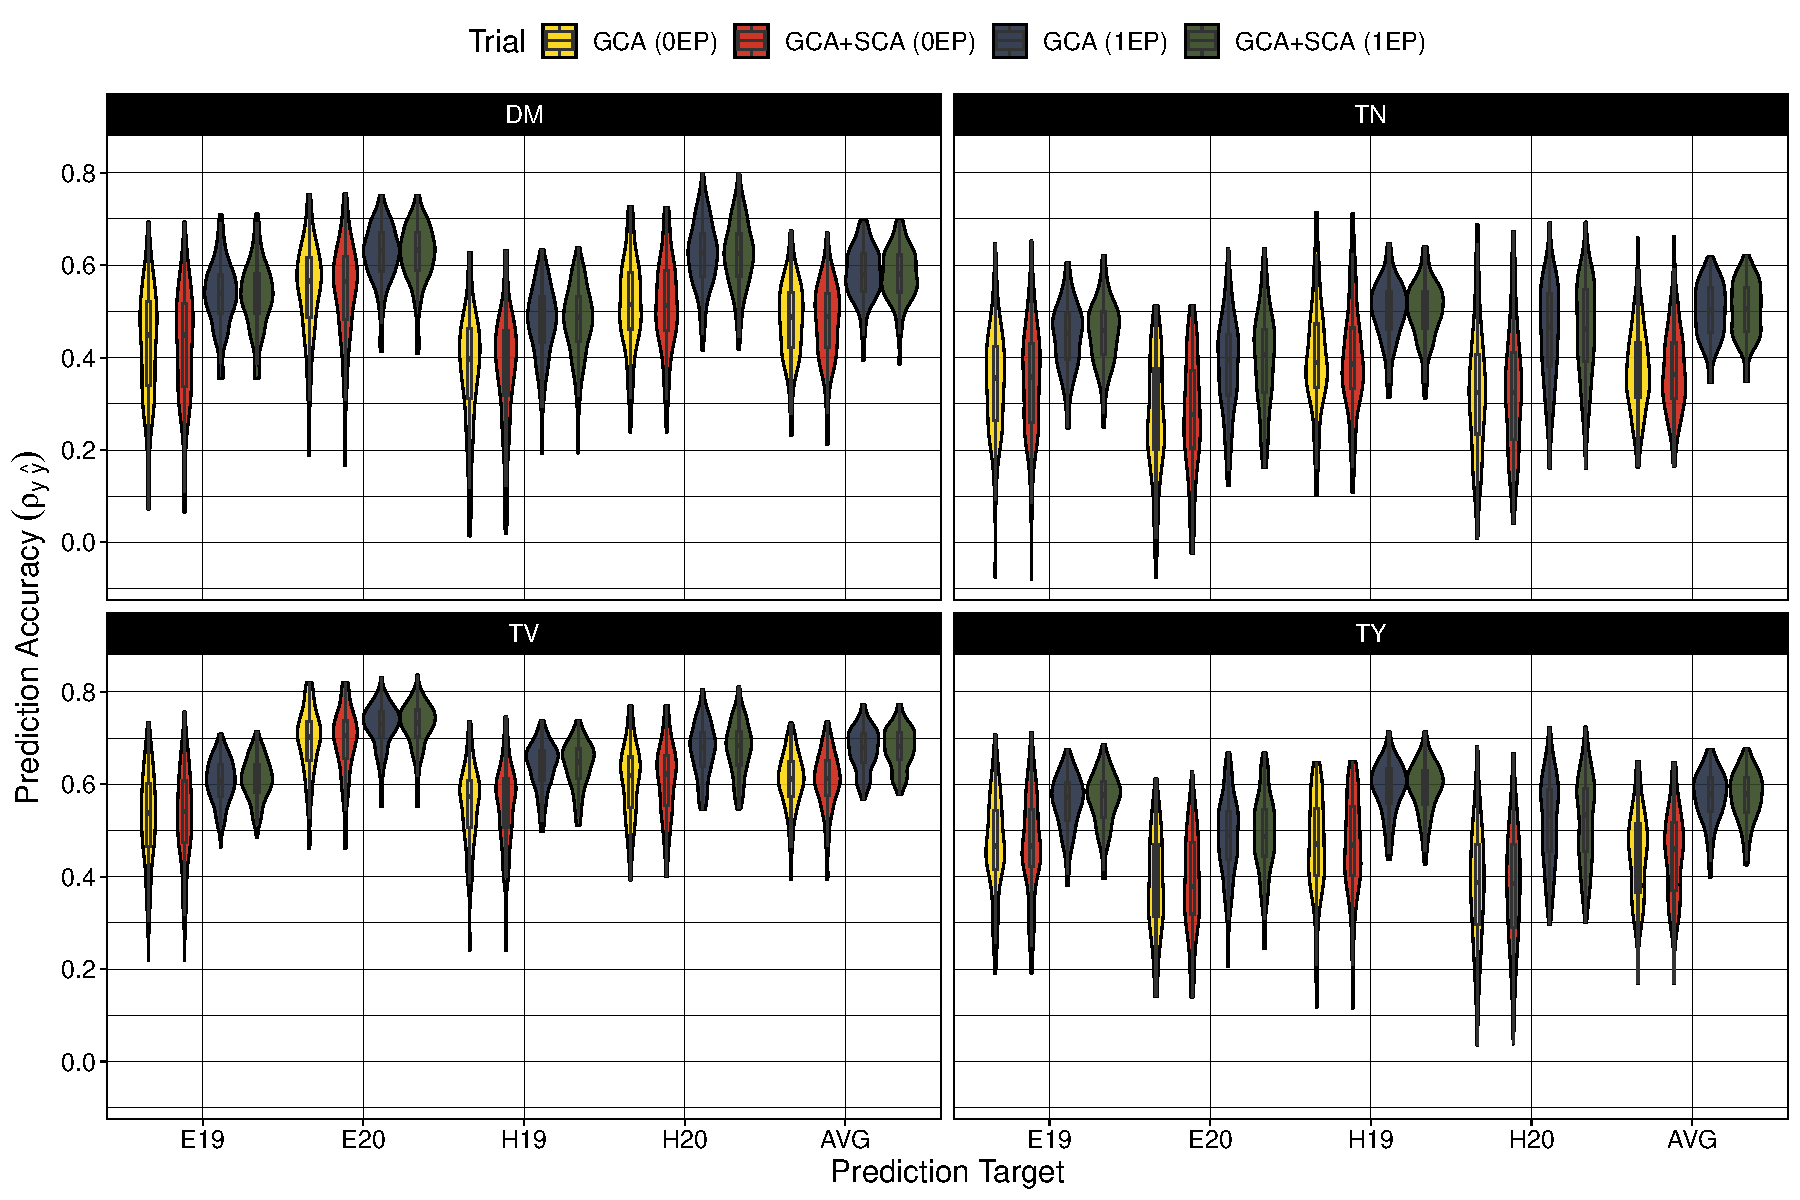
\includegraphics[width=15.5cm]{figs_03/fig-pa-1.pdf}
\end{adjustwidth}
\caption{\label{fig:pa}Predictive accuracy (correlation coefficient of true hybrid performance and predicted cross value) in the zero evaluated parent sat (0EP) and the one evaluated parent set (1EP) for GCA model and GCA+SCA models for dry matter content (DM), total tuber number (TN), mean tuber volume (TV), and total tuber yield (TY). Each trait, model, \& testing scenario were tested 100 times. Predictions were either compared to BLUEs generated from the first stage of modelling for Est 2019 and 2020 (E19 and E20, respectively) and Heelsum 2019 and 2022 (H19 and H20, respectively) or against across-trial BLUPs (AVG) produced from model \eqref{eq:multi-pheno}.}
\end{figure}


\section{Discussion}

Hybrid breeding has been revolutionized by GS and GP making adoption of these techniques a key step in accelerating quantitative improvement. Of particular importance when implementing these technologies is determining the contribution and nature of the genetic effects in the relevant target and then assessing how molecular marker and pedigree information can best provide predictive power for it. This in turn provides a roadmap for breeders to place these predictive methods where they can be most efficiently applied. Additionally, understanding the presence of genotype by environment interaction has also received increasing attention as selection continues to shift away from general performance to adaptability to specific envirotypes. Our findings represent a first inspection of GP for multiple tuber traits in hybrid potato using conventional genetic models.

\subsection{Feasability of genomic prediction in hybrid potato}

GP was possible in both testing scenarios (0EP and 1EP) in both genetic models (GCA and GCA+SCA) for all tuber traits, though not equally among them. Average tuber volume had the highest prediction accuracy in both test scenarios (0.61 \& 0.68, respectively) followed by dry matter content and total tuber yield. Looking among other available studies, dry matter content (and starch) has consistently high prediction accuracy's (0.73-0.84) in tetraploid populations \cite{Sverrisdottir2018, Cuevas2022, Ortiz2022}. Total yield (and components of yield) were more variable (0.31 - 0.66) reflecting different modelling strategies and training set properties \citep{Ortiz2022, Wilson2021}. Among our traits studied, total tuber number exhibited the poorest prediction accuracy especially in the 0EP testing scenario (Figure \ref{tbl:pa}). \citep{Wilson2021} similarly found relatively poor model performance for tuber number with their additive model showing an average accuracy of 0.35. In contrast to the tetraploid studies, our prediction accuracy's were notably lower. This can likely be attributed to differences in testing strategies and a smaller training to test set ratio (expectation of 1 and 0.5 for the 0EP and 1EP sets, respectively) resulting in a more severe testing in contrast to the K-fold cross-validation strategy invoked elsewhere.

\begin{figure}[H]
\begin{adjustwidth}{-\extralength}{0cm}
\centering
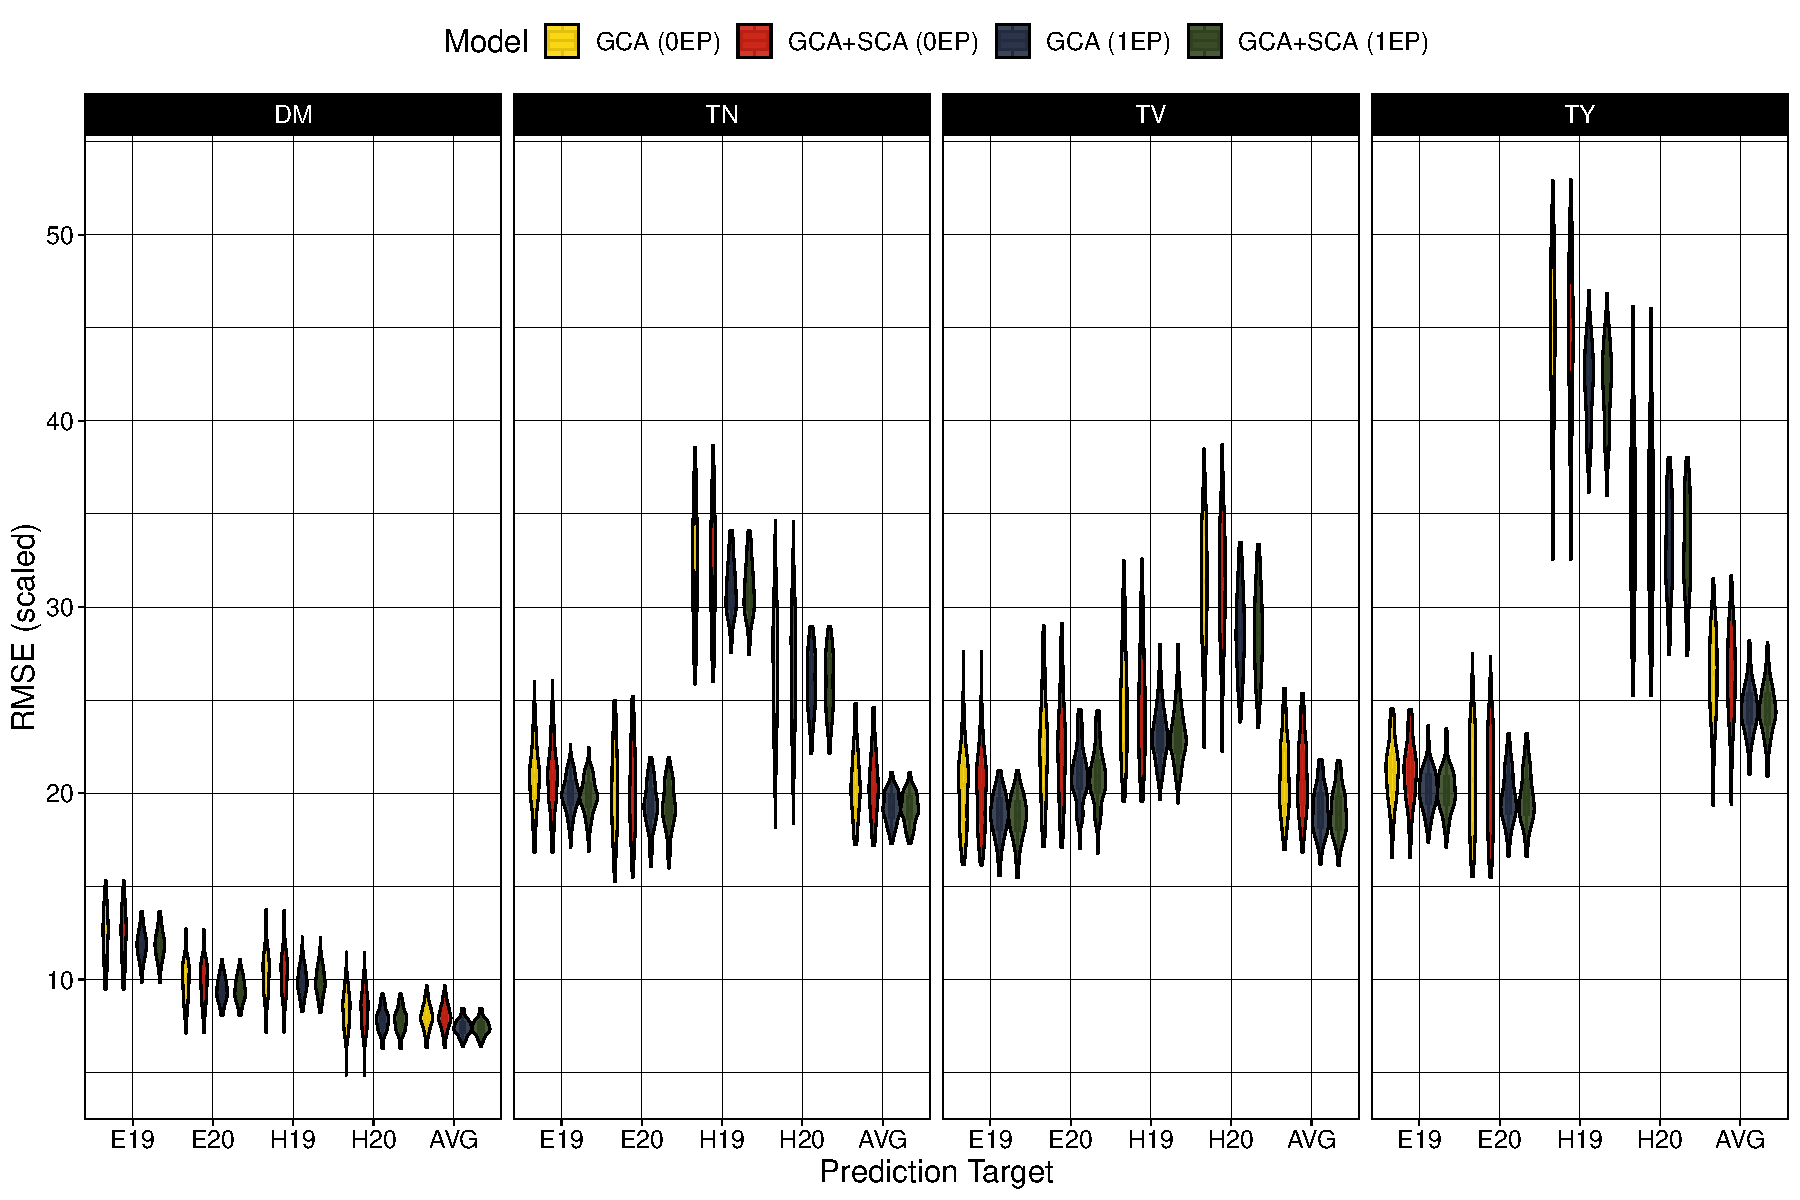
\includegraphics[width=15.5cm]{figs_03/fig-rmsd-1.pdf}
\end{adjustwidth}
\caption{\label{fig:rmsd}Scaled root mean square error (\(100\cdot\sqrt{\mathsf{E}(\hat{y}- y)^2}/\mu\)) in prediction in the zero common parent (0EP) and one common parent (1EP) sets for GCA and GCA+SCA models for dry matter content (DM), total tuber number (TN), mean tuber volume (TV), and total tuber yield (TY). Each trait, model, \& testing scenario were tested 100 times. Predictions were either compared to BLUEs generated from the first stage of modelling for Est 2019 and 2020 (E19 and E20, respectively) and Heelsum 2019 and 2022 (H19 and H20, respectively) or against across-trial BLUPs (AVG) produced from model \ref{eq:multi-pheno}.}
\end{figure}

\subsection{Contribution of non-additive effects in prediction}

We found no practical benefit in the incorporation of dominance effects (via SCA) for GP model performance in any tuber phenotype. The lack of \emph{value add} with SCA also appears inconsistent given the magnitude of SCA variances measured here (Table \ref{tbl:genmod-vars}) and in our preceding phenotypic study \cite{Adams2022}. As highlighted there, several lines of reasoning can be pursued while considering non-additive genetic effects. Reflecting on the sparse crossing design used to generate these hybrids, its not unexpected for shrinkage of the SCA effects even if the model is technically identifiable. If this is the case, then larger training sets would be required for exploitation of SCA among hybrids. Alternatively, reflecting on the size of the genetic residual (between 20 and 37\% of \(\sigma_G^2\)), kernel-based approaches could be more informative in predicting hybrid performance \cite{Gianola2008, Crossa2019a}. Rather than decomposing the total genetic value into separate additive and non-additive components, prediction is instead based upon the total observed genetic value \cite{Bernardo2020}. The application of such semi-parametric approaches could be an interesting avenue for future prediction modelling in DHP.

\subsection{Hybrid prediction and genotype by environment interaction}

While present, genotype by environment interactions did not appear to affect model performance for dry matter content and average tuber volume. This coincides with relatively consistent heritabilities between trial locations and the small \(\sigma_{gxt}^2\) variance components for both traits. Several studies in diploid \cite{Stockem2020} and tetraploid \cite{Endelman2018, Cuevas2022, Ortiz2022, Wilson2023} potato also corroborate the high stability of dry matter content. Examining total yield and tuber number, prediction accuracy's appear fairly stable across target environments, but prediction errors were highly dependent on target environment (Figure \ref{fig:rmsd}). This was especially apparent between Heelsum and Est 2019 trials where the difference in median scaled RMSE was over 25\% and 12\%, respectively. Considering the significant differences in heritabilities between trial locations (Table \ref{tbl:trait-variances}), this could negatively impact prediction accuracy if the genotype by environment structure does not reflect this. Similar to what has been reported in tetraploid \cite{Cuevas2022, Ortiz2022, Wilson2023}, total yield is highly influenced by genotype by environment interaction and difficult to structure. For future work in genotype by environment interactions, designing trials around known abiotic stresses in potato would allow for more meaningful decomposition of these effects. Doing so in climates which target relevant condition for the world's potato growers is also important in a GP context for prediction of hybrid adaptability.

\subsection{Genomic prediction for breeders}

These results have some implications for potato breeders. First, this study gives ample evidence that stable additive genetic effects are not only able to be estimated for potato inbred lines, but can also be leveraged for the prediction of a parent's breeding value in a dedicated cross. In particular, these results show the potential of genomic prediction in both a test cross and novel crossing set context through the use of the 1EP and 0EP test sets, respectively. Based upon these results, confident predictions can be offered in both contexts for all phenotypes studied here with the exception of total tuber number which exhibited depressed prediction accuracy's making them too unreliable in a novel crossing set for breeders. The GCA variance being the largest genetic effect among all traits is also worth reiterating as it directs breeders towards prioritizing additive variance among multiple tuber traits. This directly touches upon a breeding program's structure and how it exploits additive variation during population improvement among highly heritable traits. 

\section{Conclusions} % (fold)

In this study, we have laid out the groundwork for genomic prediction in hybrid potato with simple genetic models and no training set optimization. We demonstrate the GEBVs estimated from an additive model (our GCA model) suffices in predicting hybrid potato performance in dry matter content, average tuber volume, and total yield. The effect of genotype by environment interaction is mostly relevant for yield components like tuber number and total yield while dry matter content and average tuber volume were remarkably stable among target environments for genomic prediction. Principally, these results show for the first time that genomic prediction can be leveraged for inbred and hybrid selection in diploid hybrid potato. The adoption of predictive breeding in diploid potato is invaluable for the continued genetic progress of this new hybrid crop.

\funding{The research produced for this publication was made possible through funding provided by Topsector Tuinbouw \& Uitgangsmaterialen in the `Re-booting potato: enhancing the breeding of hybrid diploid potato' project (project number: TU-18155).}

\conflictsofinterest{The authors of this publication have no conflicts of interest to report related to the results of this study or the inferences, speculation,\& conclusions derived from them.}


}
\chapter[Digging up QTL: Evaluating the efficiency of marker-assisted selection in hybrid potato]{Digging up QTL: Evaluating the efficiency of marker-assisted selection in hybrid potato}
\chaptermark{Evaluating the efficiency of marker-assisted selection in hybrid potato}
\label{cha:chapter4}
\vspace*{\fill}

\newpage

\section*{Abstract}

Hybrid potato is a novel crop strategy which develops cultivars with improved F1 
hybrids created from inbred diploid potato lines. As with other crops,
the hybrid breeding system allows for greater flexibility and
potentially greater speed in contrast to traditional tetraploid potato
breeding. An important aspect of how a hybrid breeding program should be
structured is resource and technology allocation for optimum selection efficiency.
The authors of this paper examined this question with respect to marker
and selection technologies examining the relative efficiency of
marker-assisted selection (\texttt{MA}) relative to a traditional
genome-wide selection (\texttt{GW}) for F4 candidate selection. For the MA scenario, we were
able to identify 35 QTL for all tuber phenotypes that accounted for a large portion of the genetic variation in multiple yield components. The \texttt{GW} strategy
had the highest prediction accuracy with relative selection efficiency's
consistent with this for all traits. However, when examining the
relative efficiency with respect to cost of genotyping strategy, the
\texttt{MA} scenario was more efficient for all traits studied here. Our
findings suggest that marker-assisted selection could be an attractive
method for quantitative trait selection in commercial hybrid potato
programs.

\newpage

\section{Introduction}

Potato (\emph{Solanum tuberosum} L.) is the newest field crop
undergoing conversion to a hybrid breeding system
\autocite{DeVries2023,Jansky2016}. Following the success of other crops
like sugar beet \autocite{McGrath2018} and sunflower
\autocite{Dimitrijevic2018}, both private and public ventures are
endeavouring to convert this clonal tetraploid crop into a diploid
chasing the same benefits that were originally observed in maize
\autocite{Duvick1997}. This conversion in potato is actually composed of
two distinct and yet inter-related activities: (1) ploidy reduction from
a tetraploid to diploid, and (2) the shift from outcrossing populations
to structured inbred populations shaped around F1 hybrid performance.
The benefits of the former primarily lie in the ease and speed of
positive gene fixation in a disomic inheritance model over tetrasomic
inheritance \autocite{Hougas1958} with the latter comprising both
technical (trait fixation in inbreds, exploitation of heterotic vigour)
and commercial (intellectual property protection, consistent product
quality and uniformity) related advantages \autocite{Wright1980}.
Despite the allure of these propositions, it is only within the past
decade that commercialization efforts of hybrid potato programs have
come to pass due in part to overcoming genetic barriers like severe
inbreeding depression, fertility anomalies, and ploidy barriers for
secondary and tertiary gene pools
\autocite{Zhang2019,Endelman2016,Zhang2021}.

It is well understood that while hybrid breeding systems bring many
potential benefits to crop improvement strategies, this is not without
significant cost. Hybrid breeding is known to suffer from longer
breeding cycles in contrast to line breeding and necessitates specific
populations for heterotic pool development
\autocite{Labroo2021,Longin2013}. A large aspect of that complexity lies
in that the target for improvement is F1 performance and not inbred
family \emph{per se} yields due to poor correlations between the two. In
the pre-genomics era, testcross evaluation was the crux of line
advancement and population enrichment as it permitted the estimation of
general and specific combining abilities \autocite{Carangal1971}. It was
not until the advent of molecular technologies that it became possible
to develop inexpensive proxies in the place of field evaluation, first
in the form of molecular markers for marker-assisted selection (MAS) not
long followed by genome-wide regression using hundreds to thousands of
markers for genomic selection (GS) \autocite{Lande1990,Meuwissen2001}.
These methods alone have been responsible for incredible gains for
quantitative trait improvement in field and vegetable crops alike over
the past 30 years.

While genome-wide selection is a powerful tool in quantitative trait
improvement, it is not necessarily the most \emph{efficient}.
Genome-wide selection has been shown to work very well in both
tetraploid and diploid potato populations
\autocite{Adams2023,Wilson2021}, but the cost associated with training
set development, dense molecular marker panels, and computational
capacity make it a resource-intensive process. An interesting
alternative would be identifying quantitative traits which could be
selected solely on the basis of QTL information. The literature is ripe
with examples of large-effect QTL responsible for controlling traits
such as tuber shape \autocite{Eck2022}, starch content
\autocite{Li2019a}, maturity \autocite{Li2018,Massa2015} and even volume
and weight of tubers \autocite{Korontzis2020,Clot2024}. Making these
identified QTL the basis of selection in a MAS program could be a simple
and and cost-effective method for improving quantitative trait targets in
potato. However, while the success of MAS is well understood in other
crops and simulation \autocite{Podlich2004, VanBerloo2008}, its utility in hybrid
potato is currently unknown. We examine the following scenarios: a
marker-assisted breeding scenario which conducts selection based on
identified QTL in the hybrid (\texttt{MA}), a genome-wide selection
method (\texttt{GW}), and lastly a method which bases selection on 1
random SNP per chromosome (\texttt{PC}). These three strategies were
assessed on their prediction accuracy for the tuber phenotype as well as
on the relative efficiency with respect to genome-wide selection. With
these results, we hope to identify if marker-assisted selection is a
useful selection method in practice for complex traits in potato.
\section{Material and methods}

\subsection{Hybrid Phenotypic Data}\label{hybrid-phenotypic-data}

This study used a population of 785 genotyped F1 hybrids which had
undergone field evaluation between 2019 and 2020. As described in
\autocite{Adams2023}, this dataset comprises four field trials in two
trial locations (Heelsum and Est, Netherlands). Best linear unbiased
predictions (BLUPs) for hybrids were computed using the following model:

\begin{equation}\protect\hypertarget{eq-blup-model}{}{ y_{bfht} = \beta_f +\gamma_{fb} + a_{ht} + \varepsilon_{bfht} }\label{eq-blup-model}\end{equation}

where \(y\) is some component of yield for hybrid \(h\) within block
\(b\) in trial location \(t\) and specific field trial \(f\). \(y\) is
modeled on a fixed trial (\(\beta_f\)) and block within-trial
(\(\gamma_{fb}\)) effects, a random hybrid by trial (\(a_{ht}\)), and an
independent and identically distributed (IID) residual term
(\(\varepsilon_{bfht}\)). The hybrid by trial effect was modeled as
Gaussian with an unstructured variance structure:

\[a \sim \mathrm{N} \left (\mathbf{0},  \Sigma_a \right )  ~~~~~~~~~~~~~  \Sigma_a =\begin{bmatrix} \sigma^2_{\mathrm{G(Est)}} &  \sigma_{\mathrm{G(Est),G(Hee)}}\\ \sigma_{\mathrm{G(Hee),G(Est)}} & \sigma^2_{\mathrm{G(Hee)}}\end{bmatrix}\]

This model structure was chosen over simpler multi-environment models
due to large observed differences in genetic variances during
exploratory analysis. Such large discrepancies in variance were not
observed for the residual term across trials so this retained its IID
variance structure. Several variates were analyzed including including
total tuber yield (TY; \(\mathrm Mg \cdot \mathrm{Ha^{-1}}\)), tuber dry
matter content (DM; per cent), and average tuber volume (TV; \(cm^3\)).

\hypertarget{marker-processing}{%
\subsection{Marker processing}\label{marker-processing}}

Using the same dataset described in \autocite{Adams2023}, marker data
was collected on the 416 parental lines used in the creation of the
evaluated hybrids. These lines were genotyped with a targeted
genotyping-by-sequencing (GBS) technology marketed as SeqSNP and
developed by LGC \autocite{LGC2019}. For this analysis, single
nucleotide polymorphism's (SNPs) were extracted and filtered from the
probeset and filtered based upon SNP missingness, minor allele
frequency, and SNP density. These filter criteria left 1,040 remaining
SNP's which were used to infer F1 hybrid genotypes for QTL mapping and
genome-wide prediction.

\hypertarget{qtl-scanning-and-incorporation}{%
\subsection{QTL Scanning and
Incorporation}\label{qtl-scanning-and-incorporation}}

QTL scans were conducted on all phenotypes using the hybrid BLUPs
averaged over location and standard errors produced from ASReml-R's
\texttt{predict()} interface along with SNP data. This was done using a
forward-selection approach. The null model has the following form:

\begin{equation}\protect\hypertarget{eq-null-model}{}{ \hat{\mathbf{y}} = \mathbf{1}\mu + \mathrm{X_Q}\beta_{Q} + \mathrm{Z_g}u + e }\label{eq-null-model}\end{equation}

where \(\hat{\mathbf{y}}\) is the vector of hybrid predictions, \(\mu\)
is the global mean, \(\beta_Q\) is a vector of QTL fixed effects, \(u\)
is a vector of random background genetic effects
(\(u \sim \mathrm{N}(0, \sigma^2_g)\)), and \(e\) is a vector of
residuals whose variance is structured from the first-stage model
standard errors
(\(e\sim \mathrm{N}(0, \mathrm{R = Diag(\hat{se^2_1}, \hat{se^2_2}, \ldots, \hat{se^2_n})})\)).
During the first QTL scan, \(X_Q\), the design matrix which contains SNP
dosage of previously identified QTL, and \(\beta_Q\) will be empty. The
design matrix for the background genetic effects, \(\mathrm Z_g\), is a
diagonal matrix.

This model is tested against a scanning model:

\begin{equation}\protect\hypertarget{eq-scan-model}{}{ \hat{\mathbf{y}} = \mathbf{1}\mu + \mathrm{X_Q}\beta_{Q} + \mathrm{Z_g}u + \mathrm{Z_{snp}}v + e }\label{eq-scan-model}\end{equation}

which differs only in the addition of one random term, \(v\), the SNP
effect (\(v \sim \mathrm{N(0,}\sigma^2_{qtl}\)) being tested at any
given scan. The forward-selection procedure consisted of: (1) fitting
the null model in (Equation~\ref{eq-null-model}), (2) fitting the
scanning model (Equation~\ref{eq-scan-model}), (3) conducting a
likelihood ratio test to assess the significance of \(v\), (4) repeating
steps 2-3 for all remaining SNPs, (5) selecting the SNP with the
smallest p-value and placing it in \(\mathrm{X}\) if it was smaller than
the cutoff (defined by a Bonferroni threshold) and then repeating. If
there were no remaining SNPs with sufficient evidence of putative QTL,
the scan was concluded. A Wald test was then conducted on the final
model to confirm the significance of all QTL in \(\mathrm{X_Q}\); the
effect size of all QTLs were extracted from this model
(Figure~\ref{fig-snp-size}). While some QTLs clustered within close proximity to one another, all QTL distances were above 1 Mb and thus considered independent of one another. Lastly, each QTL was fit in a single QTL
model
(\(\hat{\mathbf{y}} = \mathbf{1}\mu + \mathrm{Z_g}u + \mathrm{Z_{snp}}v + e\))
to estimate the proportion of QTL variance (Figure~\ref{fig-gen-size}).

The number of QTL taken up in each model was recorded
(Table~\ref{tbl-summary}) along with their significance
(i.e.~\(- \mathrm{log}_{10}(p)\)) during initial model scanning
(Figure~\ref{fig-lod-score}). All QTL modeling and phenotypic analyses
were done using ASReml-R 4.2 \autocite{Butler2017}.

\subsection{Genomic Prediction Models}\label{genomic-prediction-models}

Because one of the major research questions was related to testing the
utility of a multi-QTL model in a marker-assisted selection program, we constructed
multiple prediction models associated with distinct modeling scenarios
(See Table~\ref{tbl-scenarios}). The first was a marker-assisted
selection model (\texttt{MA}) which bases prediction upon the previously
identified QTL (Table~\ref{tbl-summary}). All QTL which were found to be
jointly significant were incorporated into a traditional linear
regression model to predict a candidate's value among our selected
quantitative traits. This model was:

\begin{equation}\protect\hypertarget{eq-mas-model}{}{ \hat{\mathbf{y}} = \mathbf{1}\mu + \mathrm{X}_Q\beta_Q + \varepsilon }\label{eq-mas-model}\end{equation}

where the hybrid BLUPs were modeled only on the global mean, and
estimated QTL effects (\(\beta_Q\)) in each hybrid. This scenario was
contrasted against a genome-wide based regression using 1000 SNPs
(\texttt{GW}) and a model which picks one random SNP per chromosome
(\texttt{PC}). The latter is meant to perform as a negative control to
evaluate the minimum performance threshold from a SNPs linkage within a
linkage group. Both of these models were trained using ridge
regression and could be expressed as:

\begin{equation}\protect\hypertarget{eq-rr-model}{}{ \hat{\mathbf{y}} =  \mathbf{1}\mu + \mathrm{W}u + \varepsilon }\label{eq-rr-model}\end{equation}

where the SNP dosages are contained in matrix, \(\mathrm{W}\), and all
marker effects in \(u\). To assess prediction performance, all models
were tested using 5-fold cross-validation. Cross-validation was
replicated 100 times for each trait for the \texttt{MA} model and
Pearson correlation coefficients were estimated for each fold and then
averaged over each replicate. For models which introduced marker
sampling variation (i.e., \texttt{GW} and \texttt{PC}), the replication
was stratified over marker sampling (\(n = 20\)) and fold partitioning
of hybrids (\(m = 50\)) for a total of 1000 replications. Similarly,
the predictive performance was assessed via the Pearson correlation
coefficient between the true and predicted hybrid performance and
averaged over each fold. The average Pearson correlation coefficient
were then compared across all models and traits (Figure~\ref{fig-pa}).
All prediction models were trained and tested used the
\texttt{mixed.solve()} function provided through the rrBLUP R library
\autocite{Endelman2011}.

\hypertarget{tbl-scenarios}{}
\begin{longtable}[]{@{}
  >{\raggedright\arraybackslash}p{(\columnwidth - 8\tabcolsep) * \real{0.0952}}
  >{\raggedright\arraybackslash}p{(\columnwidth - 8\tabcolsep) * \real{0.3333}}
  >{\raggedright\arraybackslash}p{(\columnwidth - 8\tabcolsep) * \real{0.1905}}
  >{\raggedright\arraybackslash}p{(\columnwidth - 8\tabcolsep) * \real{0.1905}}
  >{\raggedright\arraybackslash}p{(\columnwidth - 8\tabcolsep) * \real{0.1905}}@{}}
\caption{\label{tbl-scenarios}Breeding scenarios with descriptions of
model parameters and cost associated with each.}\tabularnewline
\toprule\noalign{}
\begin{minipage}[b]{\linewidth}\raggedright
Scenario code
\end{minipage} & \begin{minipage}[b]{\linewidth}\raggedright
Scenario
\end{minipage} & \begin{minipage}[b]{\linewidth}\raggedright
\(\hat{\beta}\)
\end{minipage} & \begin{minipage}[b]{\linewidth}\raggedright
\(\hat{u}\)
\end{minipage} & \begin{minipage}[b]{\linewidth}\raggedright
Cost
\end{minipage} \\
\midrule\noalign{}
\endfirsthead
\toprule\noalign{}
\begin{minipage}[b]{\linewidth}\raggedright
Scenario code
\end{minipage} & \begin{minipage}[b]{\linewidth}\raggedright
Scenario
\end{minipage} & \begin{minipage}[b]{\linewidth}\raggedright
X
\end{minipage} & \begin{minipage}[b]{\linewidth}\raggedright
W
\end{minipage} & \begin{minipage}[b]{\linewidth}\raggedright
Cost
\end{minipage} \\
\midrule\noalign{}
\endhead
\bottomrule\noalign{}
\endlastfoot
MA & Marker-assisted selection with identified QTLs & Identified QTL & &
\$0.15 per SNP per sample \\
GW & Genome-wide regression using mid-sized probe set & global mean &
1000 genome-wide SNP's & \$150.00 per sample \\
PC & Selection with one random SNP on each chromosome & global mean & 1
SNP per chromosome & \$1.80 per per sample \\
\end{longtable}

Putting the model performance in the context of a breeding program, we
examine \texttt{MA}, \texttt{PC}, and \texttt{GW} as alternative
modeling methods for predicting the genetic value of 1000 novel F4
candidates for creating superior F1 candidates. This is done on the basis of marker effect estimation at the F1 hybrid level which would make inbred selection based on that line's geonmically estimated breeding value. These schemas were evaluated
based on the relative efficiency for the \texttt{MA} and \texttt{PC}
scenarios relative to \texttt{GW} (Table~\ref{tbl-scenarios}). This is
the ratio of the predicted selection response (\(i\sigma_gr\)) of each
scenario over the genome-wide regression scenario \autocite{Krchov2015}.
Because the only difference between these scenarios is in the selection
accuracy (\(r\)), the relative efficiency is then just the ratio of the
selection accuracy from each scenario. This was extended further through
the inclusion of genotyping costs of the 1000 candidates for each
strategy assuming a SNP assay genotyping method. This was done by
dividing the predicted selection response of each strategy by the log of
the genotyping cost. While costs vary according to locale, number of
samples, and specific technology, we chose pricing that appeared
reasonable given trends over the past decade \autocite{Semagn2014}.
Therefore, each scenario was assessed with respect to the relative
efficiency and the relative efficiency divided by the log of the
genotyping costs (Table~\ref{tbl-re}).

\begin{figure}

{\centering 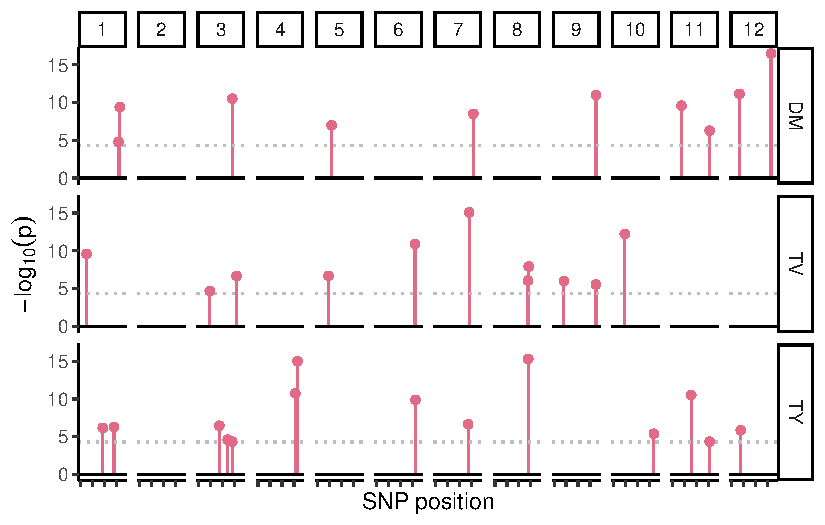
\includegraphics{figs_04/fig-lod-score-1.pdf}

}

\caption{\label{fig-lod-score}The physical positions and \(log_{10}\)
probabilities found for all 39 QTL across potato genome for dry matter
content (DM), tuber volume (TV), and total tuber yield (TY).}

\end{figure}
\section{Results}

\subsection{QTL Scan}\label{qtl-scan}

All scanning models converged successfully and picked up multiple QTL
for each phenotype (Table~\ref{tbl-summary}). The final QTL models
exhibited a better goodness of fit in contrast to the null model. This
was reflected both in the change of the AIC as well as reduction in
background genetic variance in each final model, though, this was trait
dependent. Between 53 and 56\% of the genetic variance was partitioned
away from the background genetic term between the null and final model
across traits. Among the traits tested, dry matter content appeared to
improve most through the incorporation of the 10 identified QTL
(Table~\ref{tbl-summary}).

In total, 35 QTL peaks were detected but given overlap between traits,
this comprised 33 unique QTL (Table~\ref{tbl-summary}). Total tuber
yield detected the largest number of QTLs (14 QTL) with tuber volume and
dry matter content detecting 11 and 10, respectively. The QTL variance
varied between 10 and 62\% of the total genetic variance among all
phenotypes but the median proportion of variance was highest in
drymatter content (36.0\%) followed by total tuber yield (30.1\%) and
average tuber volume (29\%) (Figure~\ref{fig-gen-size}). There were multiple QTL clusters detected for all three phenotypes comprising chromosome 1 for
dry matter content (chr01:83523334 and chr01:86604310), chromosome 8 in
tuber volume (chr08:46811267 and chr08:47889222), chromosome 4 in total
yield (chr04:60035708 and chr04:64373508).

\hypertarget{tbl-summary}{}
\begin{table}
\caption{\label{tbl-summary}Model parameters for the null and final QTL models for dry matter
content (DM), average tuber volume (TV) and total tuber yield (TY). The
Akaike Information Criterion (AIC), the change in AIC (\(\Delta AIC\)),
background genetic variance (\(\sigma^2_g\)), and per cent change in
background genetic variance (\(\Delta \% \)) for the initial
null and full QTL models. This is presented with the estimated global
mean of each trait and the total number of QTL incorporated into the
final model. }\tabularnewline

\centering
\begin{tabular}{ccccccccc}
\toprule
\multicolumn{1}{c}{ } & \multicolumn{3}{c}{AIC} & \multicolumn{3}{c}{$\sigma^2_g$} & \multicolumn{2}{c}{ } \\
\cmidrule(l{3pt}r{3pt}){2-4} \cmidrule(l{3pt}r{3pt}){5-7}
Phenotype & Null model & Final model & $\Delta$ & Null model & Final model & $\Delta\%$ & $\mu$ & Number of
QTL\\
\midrule
DM & 1690.0 & 1299.1 & 390.9 & 2.5 & 1.2 & 52.9 & 20.7 & 10\\
TV & 3650.0 & 3115.7 & 534.3 & 35.7 & 15.6 & 56.4 & 29.9 & 11\\
TY & 3394.1 & 2913.8 & 480.4 & 24.6 & 11.1 & 54.6 & 14.5 & 14\\
\bottomrule
\end{tabular}
\end{table}

\begin{figure}

{\centering 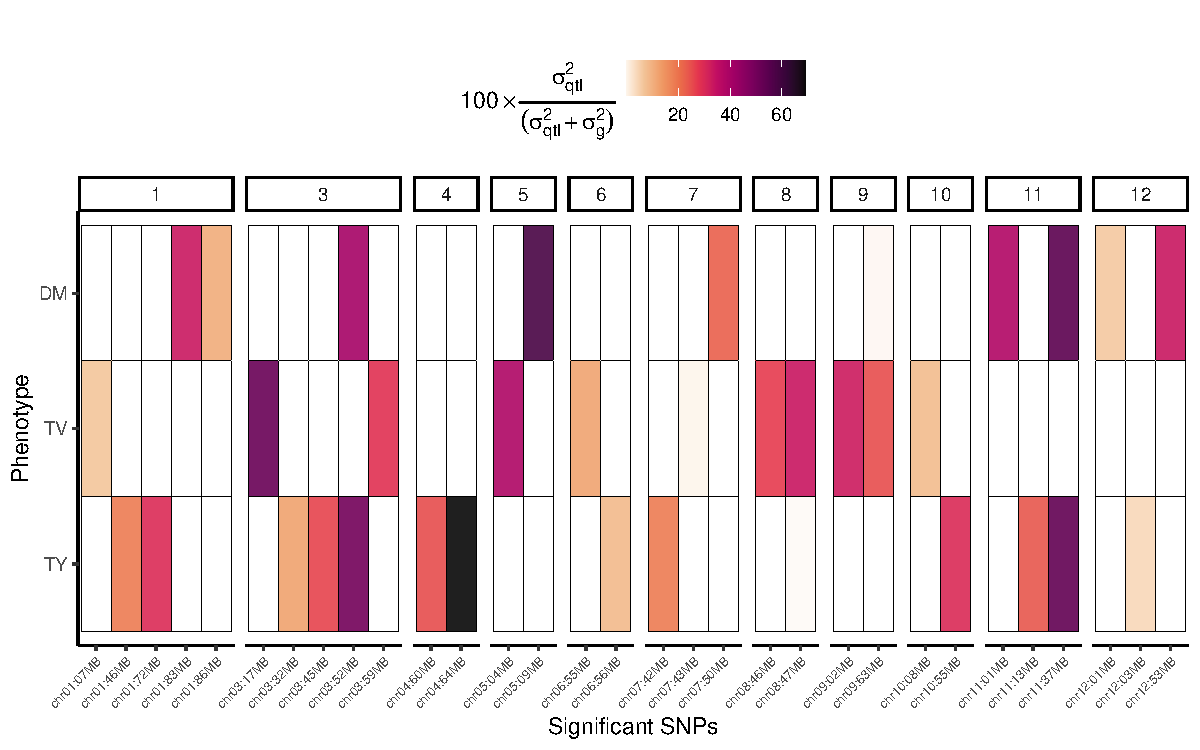
\includegraphics{figs_04/fig-gen-size-1.pdf}

}

\caption{\label{fig-gen-size}Proportion of captured genetic variance
from each QTL in the scanning model among all 35 identified QTL separated per chromosome in dry
matter content (DM), average tuber volume size (TV), and total tuber
yield (TY).}

\end{figure}

Examining all detected QTL, varying QTL effect size was observed with
respect to magnitude and direction (Figure~\ref{fig-snp-size}). The
largest QTL effects were observed in total tuber yield with effects as
large as 30\% of the mean. The QTL observed in dry matter content also
tended to be smaller in magnitude than those observed in tuber volume
and total tuber yield. Two correlated QTL were observed for dry matter
content and total tuber yield on chromosome 3 (chr03:52583805) and on
chromosome 11 (chr11:37618884) (Figure~\ref{fig-lod-score}). Both QTLs
had a relatively large QTL variance (Figure~\ref{fig-gen-size}) and were
negatively correlated between total tuber yield and dry matter content
(Figure~\ref{fig-snp-size}).

\begin{figure}

{\centering 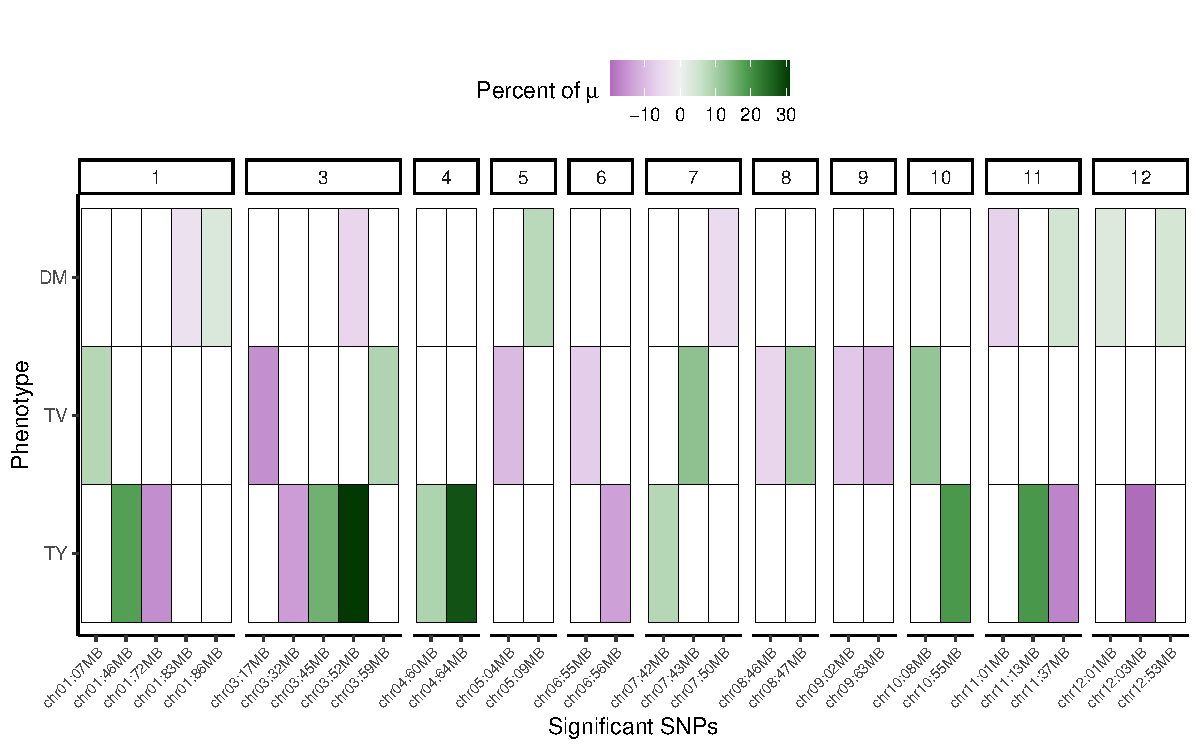
\includegraphics{figs_04/fig-snp-size-1.pdf}

}

\caption{\label{fig-snp-size}Marker effect size in \(\beta_{qtl}\) from
the final QTL model among all 35 identified QTL seperated per chromosome in dry matter content
(DM), average tuber volume size (TV), and total tuber yield (TY).}

\end{figure}

\begin{figure}

{\centering 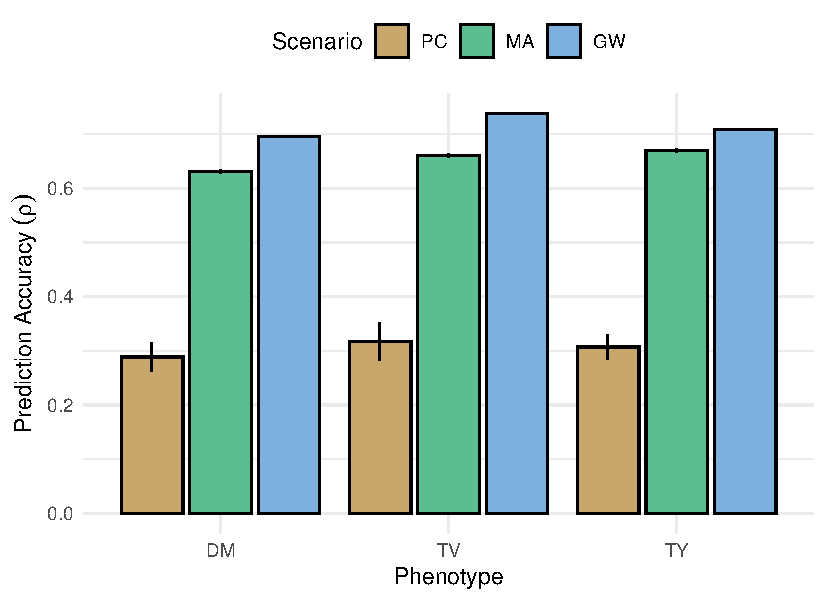
\includegraphics{figs_04/fig-pa-1.pdf}

}

\caption{\label{fig-pa}Prediction accuracy results from 5-fold cross
validation for qtl mapping (qtl), genome-wide regression (GW), and
marker-assisted selection with 12 random SNPs (PC). Error bars contain
one standard deviation around the average Pearson correlation
coefficient.}

\end{figure}

\hypertarget{genomic-prediction-models-1}{%
\subsection{Genomic Prediction
Models}\label{genomic-prediction-models-1}}

Turning to each predictive strategy, the \texttt{GW} scenario performed
consistently better than all other strategies and represented the maximum
prediction potential that could be attained (Figure~\ref{fig-pa}). It
also appears to closely mirror the phenotype heritabilities and
performance observed in previous studies (See \textcite{Adams2023}).
Conversely, the model used in \texttt{PC} were consistently the worst
performing with observed prediction accuracy's between 0.24 and 0.34 across
phenotypes. The \texttt{MA} models not only surpassed the negative
control (\texttt{PC}), but followed closely with the performance
observed in the \texttt{GW} model with \(\rho\)'s between 0.53 and 0.68
across traits. The \texttt{PC} strategy had the highest variability in
\(\rho\) during cross-validation due likely to the large probe sampling
variance. Examining these results relative to the \texttt{GW} scenario,
\texttt{MA} had a far larger relative efficiency for the three traits
targets (0.89 - 0.95) in contrast to \texttt{PC} (0.42 - 0.43)
(Table~\ref{tbl-re}). Looking to genotyping costs, the cost ratios varied very little between \texttt{MA} and \texttt{PC} strategies; both strategies were within two orders of magnitude cheaper than the \texttt{GW} genotyping strategy. All relative efficiencies were less than 1 but
when genotyping costs were considered, the \texttt{MA} was considerably
higher for all traits (1.41 - 1.48) indicative of higher selection
efficiencies per log cost. This was in contrast to the \texttt{PC}
scenario which had very low relative efficiency per log cost.
\section{Discussion}

An important exercise for any breeding program is the careful analysis
of goals for trait improvement in light of the genetic variation
present, the statistical architecture of the trait, and available
resources available to a program. Examining the
particular question of genotyping technology and selection methods, we
provide a template for evaluating the efficiency of breeding strategies.
In this paper, we were able to detect multiple QTL which captured a
large portion of the genetic variance in multiple tuber phenotypes. The
merit of these QTL were then tested through against a genome-wide
regression strategy and a random marker-based selection strategy as a
negative control. Selection responses were examined for all scenarios
with respect to unit gain and unit gain per unit cost. This represents
an invaluable procedure for assessing the benefits of two selection
methods in an operational breeding program.

\hypertarget{selecting-quantitative-traits}{%
\subsection{Selecting Quantitative
traits}\label{selecting-quantitative-traits}}

The first criteria for the success of quantitative trait selection is the
degree of genetic variability for the trait in question, in other words, 
the trait's heritability. Based upon the results of this study and previous
works \autocite{Adams2022} we know that all phenotypes studied here are highly
heritable and capable of genetic improvement. Based on prediction 
accuracy (Figure~\ref{fig-pa}) and consideration of
selection costs (Table~\ref{tbl-re}), we found credible evidence that
both MAS and genome-wide selection would be successful selection methods
for the traits studied here. Regarding genome-wide selection, this was in line with what other studies have observed for
these traits in potato \autocite{Adams2023,Wilson2021}. However, the
efficiency of the \texttt{MA} strategy for quantitative trait selection
needs further consideration. While MAS is an older technology and prone to lower selection accuracy's, it is still potentially an effective selection method
if sufficient genetic variation can be found. In our QTL mapping
procedure, over half the genetic variation was accounted for in the
final QTL model, and yet, the relative efficiency was as high as 0.95.
This could be a consequence of incorporating large effect QTL which
carry most of the relevant information for prediction. This was in
contrast to the \texttt{PC} control which, while having a similar number
of SNPs used for selection, offered little in way of selection
response. So given that there are still large effect QTL segregating
among candidates, the \texttt{MA} strategy is suitable in selection if
well designed markers are being used.

\hypertarget{tbl-re}{}
\begin{table}
\caption{\label{tbl-re}The relative efficiency (RE), genotyping cost ratio (CR) and relative efficiency per log cost
(\(\mathrm{RELC}\)) for the marker-assisted selection (MA) and the
single marker per chromosome strategies (PC) relative to the genome-wide
selection scenario (GW) for dry matter content (DM), average tuber
volume (TV), and total tuber yield (TY). }\tabularnewline

\centering
\begin{tabular}{ccccccc}
\toprule
\multicolumn{1}{c}{ } & \multicolumn{3}{c}{MA} & \multicolumn{3}{c}{PC} \\
\cmidrule(l{3pt}r{3pt}){2-4} \cmidrule(l{3pt}r{3pt}){5-7}
Phenotype & RE & CR & $\mathrm{RELC}$ & RE & CR & $\mathrm{RELC}$\\
\midrule
DM & 0.91 & 0.010 & 1.48 & 0.42 & 0.012 & 0.66\\
TV & 0.89 & 0.013 & 1.41 & 0.43 & 0.012 & 0.68\\
TY & 0.95 & 0.014 & 1.47 & 0.43 & 0.012 & 0.69\\
\bottomrule
\end{tabular}
\end{table}

\hypertarget{mas-versus-genome-wide-selection-costs-and-complexity}{%
\subsection{MAS versus genome-wide selection: Costs and
complexity}\label{mas-versus-genome-wide-selection-costs-and-complexity}}

When considering which of these strategies would be more appropriate for
employing in a hybrid potato breeding program, multiple questions need
to be considered. Most of these center around the maturity of the
breeding program and the priority of targets. Most crop breeding
programs are more conservative with genetic variation loss, and
therefore, would likely utilize a selection strategy which guarantees
the highest selection accuracy possible
\autocite{Swarup2021,Rasmusson1997}. In the context of these two tested
scenarios (\texttt{MA} and \texttt{GW}), this would lean towards the
genome-wide prediction approach. However, there are other programs that
could be less risk-adverse with regard to loss of genetic variation so
long as it allows for selection response (or unit selection response per
unit cost) to be maximized by some other means. We observed that when
considering genotyping costs, the \texttt{MA} strategy was more
efficient per log cost for all three trait targets (Table~\ref{tbl-re}).
When a cost penalty is introduced, any affordable technology that
borders with the performance of genome-wide regression becomes
immediately interesting for adoption. So for breeding programs which
value greater or more cost-efficient short-term gains, a marker-assisted
selection approach is worth consideration for quantitative trait
selection.

\hypertarget{operational-considerations}{%
\subsection{Operational
considerations}\label{operational-considerations}}

These scenarios are presented as is with no formal consideration of
other operational questions which could be relevant for their effective
adoption. For example, we used a population where QTLs could be
identified, however, this is of course not guaranteed. The success of
QTL identification in a breeding program is dependent on many
interrelated questions: population mapping or family mapping
\autocite{Wurschum2012}, having dedicated mapping populations or using
extant material, and the number of individuals used
\autocite{Lande1990}. Even after QTL identification, there are common
pitfalls in maintaining a marker in a MAS program such as recombination
between the QTL and marker, ensuring universal probe annealing across
relevant genetic backgrounds, and maintaining these targets alongside
other important genes necessary for a candidate's portfolio. Genome-wide
prediction methods in this regard, are more straightforward, as model
training, testing, validation, and retraining are regular procedures as
breeding populations develop over time. However, an unappreciated
logistical challenge with such predictive workflows is proper investment
in data management and well engineered data pipelines as the size of
datasets accumulate each year. The creation and maintenance of such
digital infrastructure for genomic workloads requires expertise outside
of the genetical and statistical domain and could be a liability if not
sufficiently planned accordingly \autocite{ODriscoll2013,Mulder2017}.

\section{Conclusions} % (fold)

Complex traits in field crops include some of the most economically
valuable targets for trait improvement such as biomass partitioning, abiotic
stress resistance, and crop yield. Therefore, identifying schema which
maximize the rate of genetic progress in candidate selection is an
indispensable activity for breeding programs. Here we focused our attention 
on three important yield phenotypes in potato and found that MAS could serve
as an affordable selection methodology in the place of genome-wide predictive
methods. Such a low-cost technology lends itself to allocation bottlenecks common
to breeding programs where the number of candidates are large, a scenario common to 
multiple stages of a hybrid breeding program. Tools like MAS are thus still a valuable part of the
 breeders toolbox for genetic improvement in hybrid potato.

\include{05_chapter5}
\chapter[Synthesis]{Synthesis}
\chaptermark{Synthesis}
\label{cha:Chapter6}
\newpage

“A machine does not care”
― Tom Godwin, The Cold Equations

Lorem ipsum dolor sit amet, consectetur adipisicing elit, sed do eiusmod
tempor incididunt ut labore et dolore magna aliqua. Ut enim ad minim veniam,
quis nostrud exercitation ullamco laboris nisi ut aliquip ex ea commodo
consequat. Duis aute irure dolor in reprehenderit in voluptate velit esse
cillum dolore eu fugiat nulla pariatur. Excepteur sint occaecat cupidatat non
proident, sunt in culpa qui officia deserunt mollit anim id est laborum.
 % Discussion


\backmatter
\bibliographystyle{model5-names}
\phantomsection
\addcontentsline{toc}{chapter}{References}
\bibliography{library}
\fancyhead{}

\cleardoublepage
\phantomsection

%% Back Matter
\phantomsection
\chapter{About the author}

Lorem ipsum dolor sit amet, consectetur adipisicing elit, sed do eiusmod
tempor incididunt ut labore et dolore magna aliqua. Ut enim ad minim veniam,
quis nostrud exercitation ullamco laboris nisi ut aliquip ex ea commodo
consequat. Duis aute irure dolor in reprehenderit in voluptate velit esse
cillum dolore eu fugiat nulla pariatur. Excepteur sint occaecat cupidatat non
proident, sunt in culpa qui officia deserunt mollit anim id est laborum. Lorem ipsum dolor sit amet, consectetur adipisicing elit, sed do eiusmod
tempor incididunt ut labore et dolore magna aliqua. Ut enim ad minim veniam,
quis nostrud exercitation ullamco laboris nisi ut aliquip ex ea commodo
consequat. Duis aute irure dolor in reprehenderit in voluptate velit esse
cillum dolore eu fugiat nulla pariatur. Excepteur sint occaecat cupidatat non
proident, sunt in culpa qui officia deserunt mollit anim id est laborum.


\section*{Peer-reviewed journal publications}

% Full citation of publication 1
% This refers to the article key in the refs.bib file.
\bibentry{Adams2022}

Full citation of publication 2


\section*{Peer-reviewed book chapter}

Book chapter 1

Book chapter 2

\section*{Other scientific publications}

Conference publication 1

Conference publication 2

\cleardoublepage
\phantomsection

\include{08_TESF}

\renewcommand{\headrulewidth}{0pt}
\cleartoleftpage

\include{09_funding}

\addcontentsline{toc}{chapter}{Acknowledgements}
\chapter*{Acknowledgements}

Lorem ipsum dolor sit amet, consectetur adipisicing elit, sed do eiusmod
tempor incididunt ut labore et dolore magna aliqua. Ut enim ad minim veniam,
quis nostrud exercitation ullamco laboris nisi ut aliquip ex ea commodo
consequat. Duis aute irure dolor in reprehenderit in voluptate velit esse
cillum dolore eu fugiat nulla pariatur. Excepteur sint occaecat cupidatat non
proident, sunt in culpa qui officia deserunt mollit anim id est laborum. Lorem ipsum dolor sit amet, consectetur adipisicing elit, sed do eiusmod
tempor incididunt ut labore et dolore magna aliqua. Ut enim ad minim veniam,
quis nostrud exercitation ullamco laboris nisi ut aliquip ex ea commodo
consequat. Duis aute irure dolor in reprehenderit in voluptate velit esse
cillum dolore eu fugiat nulla pariatur. Excepteur sint occaecat cupidatat non
proident, sunt in culpa qui officia deserunt mollit anim id est laborum. Lorem ipsum dolor sit amet, consectetur adipisicing elit, sed do eiusmod
tempor incididunt ut labore et dolore magna aliqua. Ut enim ad minim veniam,
quis nostrud exercitation ullamco laboris nisi ut aliquip ex ea commodo
consequat. Duis aute irure dolor in reprehenderit in voluptate velit esse
cillum dolore eu fugiat nulla pariatur. Excepteur sint occaecat cupidatat non
proident, sunt in culpa qui officia deserunt mollit anim id est laborum.


\cleardoublepage


woah its me


\end{document}
